
\documentclass{beamer}
\usetheme{default}
\setbeamertemplate{navigation symbols}{}
%	
\usepackage{subfig}
\usepackage{amsmath, amsthm, amssymb}
\usepackage{float}
\usepackage{rotating}
\usepackage{graphicx}
\usepackage{epstopdf}
\usepackage{longtable}
\usepackage{xcolor}
\usepackage{bm}
\usepackage{tikz}
\usetikzlibrary{shapes}
\tikzset{My Arrow Style/.style={single arrow, fill=red!50, anchor=base, align=center,text width=.5cm,rotate =270}}
\newcommand{\MyArrow}[2][]{\tikz[baseline] \node [My Arrow Style,#1] {#2};}
\tikzset{My 2Arrow Style/.style={single arrow, fill=red!50, anchor=base, align=center,text width=.5cm,rotate =90}}
\newcommand{\MyArrowUp}[2][]{\tikz[baseline] \node [My 2Arrow Style,#1] {#2};}
%\newcommand{at}{\begin{matrix}}
%\newcommand{\emat}{\end{matrix}}
\newcommand{\EE}{\mathbb E}

\newtheorem{acknowledgement}[theorem]{Acknowledgement}
\newtheorem{algorithm}[theorem]{Algorithm}
\newtheorem{assumption}{Assumption}
\newtheorem{axiom}{Axiom}
\newtheorem{case}[theorem]{Case}
\newtheorem{claim}[theorem]{Claim}
\newtheorem{conclusion}[theorem]{Conclusion}
\newtheorem{condition}[theorem]{Condition}
\newtheorem{conjecture}{Conjecture}
\newtheorem{criterion}[theorem]{Criterion}
\newtheorem{proposition}{Proposition}
\newtheorem{summary}[theorem]{Summary}
\newtheorem{exercise}{Exercise}
\newtheorem{notation}{Notation}
\newtheorem{remark}{Remark}
%\graphicspath{{graphs//}}

\title {Optimal Taxation with Incomplete Markets}
\author{Anmol Bhandari, David Evans, Mikhail Golosov, Thomas J. Sargent}

\date{October 2013}
% \today will show current date.
% Alternatively, you can specify a date.
%
\begin{document}
%
\begin{frame}
\titlepage

\end{frame}
\section{Introduction}
\subsection{}

\begin{frame}{Lucas and Stokey, 1983}

\begin{quote}
$\ldots$ the option to issue state-contingent debt is important: tax policies that
are optimal under uncertainty have an essential `insurance' aspect to them.
\end{quote}
\end{frame}

\begin{frame}
\frametitle{Commitment, representative agent, no capital}

\begin{itemize}

 \item \textbf{Incomplete markets}

 \quad \color{red}$\rightarrow$ \color{black} A single, possibly risky asset

 \item \textbf{Linear tax schedules}

 \quad \color{red}$\rightarrow$ \color{black}Proportional tax on labor earnings (maybe plus  {\em nonnegative} transfers)

 \item \textbf{Aggregate shocks}

 \quad \color{red}$\rightarrow$ \color{black} To productivities, government expenditures

 \end{itemize}
\end{frame}



\begin{frame}
\frametitle{Questions}

\begin{enumerate}
\item Should a  government accumulate or decumulate assets?
\item Why might different governments want to issue different amounts of debt?
\item Existing answers hinge on polar assumptions:
\begin{itemize}
 \item [+] Complete markets, Lucas Stokey (1984): non history dependent debt quantities inherited from initial condition
 \item [+ ] A risk-free bond only, quasi-linear preferences, AMSS (2002): govt. accumulates {\em assets} sufficient to finance activities using interest revenues
\end{itemize}
\item Unknown: what if interest rates fluctuate?
\end{enumerate}
\end{frame}

%
%\begin{frame}
%\frametitle{Our analysis}
%
%\begin{enumerate}
%\item \textbf{Asset structure}
%\begin{itemize}
%\item [+] A single asset only
%\item [+] We exogenously restrict asset payoffs
%
%% $\Longrightarrow$ E.g., bonds that pay less during adverse times
%
% \end{itemize}
%\item \textbf{Economic forces}
%\begin{itemize}
%\item Asset {\color{black} \textbf{levels} } can help smooth tax distortions {\color{black} \textbf{ across  states}}
%\item This differs from the  role of debt in previous incomplete markets  economies where { \color{black} \textbf{changes}} in debt levels help smooth tax distortions {\color{black}  \textbf{ over  time}}
%\end{itemize}
%\end{enumerate}
%
%\end{frame}


\section{Environment}
\subsection{}

\begin{frame}
 \frametitle{Environment}
 \begin{itemize}
 \item \textbf{Uncertainty}: Markov aggregate shocks $s_t\in \mathcal{S}$; $S \times S$ stochastic matrix $\Pi$; $g_t=g(s_t);\theta_t=\theta(s_t)$
  \item \textbf{Demography}: Infinitely lived representative agent plus a benevolent planner
  \item \textbf{Preferences }(representative household)
  \begin{equation*}
\mathbb{E}_{0}\sum_{t=0}^{\infty } \beta^t  U\left(
c(s^t),l(s^t)\right)  \label{utility lifetime}
\end{equation*}%
  \item \textbf{Technology}: Aggregate output  $y_t=\theta_{t} l_{t}$
   \end{itemize}

\end{frame}

\begin{frame}
 \frametitle{Environment, II}
 \begin{itemize}
\item \textbf{Asset market}:
\begin{itemize}
 %\item A single asset
\item $S \times S$ matrix $\mathbb{P}$ with time $t$ payoff being
\[p_t=\mathbb{P}(s_{t}|s_{t-1})\]
\end{itemize}



  \item \textbf{Linear Taxes}: Agent $i$'s tax bill
\[- T_t + \tau_t \theta_{t}l_{t},  \ T_t \geq 0 \]

\item[]
  \item \textbf{Budget constraints} $q_t$ is price of  asset

  \begin{itemize}
   \item Household: $ c_{t}+b_{t}=\left( 1-\tau _{t}\right) \theta _{t}l_{t}+\frac{p_{t}}{q_{t-1}}b_{t-1}+T_{t}$ % \ T_t \geq 0$
  \item Government: $g_{t}+B_{t}+T_t=\tau _{t}\theta_{t}l_{t}+\frac{p_{t}}{q_{t-1}}B_{t-1} $% \ T_t \geq 0$
  \end{itemize}

\item[]
  \item \textbf{Market Clearing}
  \begin{itemize}
   \item Goods: $c_{t}+g_t = \theta _{t} l_{t}$

   \item Assets: $b_{t}+B_{t}=0$
\end{itemize}
  \item[]

\item \textbf{Initial conditions}: Assets $b_{-1}, B_{-1}$ and  $s_{-1}$
\end{itemize}

\end{frame}

\begin{frame}
 \frametitle{Ramsey Problem}

\begin{definition}
\textbf{Allocation, price system, government policy}

\end{definition}

\begin{definition}
\textbf{Competitive equilibrium}: Given $\left(b_{-1},B_{-1},s_{-1}\right) $ and $\left\{ \tau _{t},T_{t}\right\} _{t=0}^{\infty }$,
all allocations are individually rational, markets clear \footnote{Usually, we impose only  ``natural'' debt limits. }
\end{definition}

\begin{definition}
\textbf{Optimal competitive equilibrium}: A welfare-maximizing competitive
equilibrium for a given $\left( b_{-1},B_{-1},s_{-1}\right) $
\end{definition}

 \end{frame}

\begin{frame}
  \frametitle{Ramsey problem}

  \begin{enumerate}
  \item \textbf{Primal approach}: To eliminate tax rates and prices, use  household's first order conditions:
\begin{subequations}
	\[
		U_{c,t} q_t = \beta \EE_t p_{t+1}U_{c,t+1}
	\]
	\[
		(1-\tau_t)\theta_tU_{c,t} = - U_{l,t}
	\]
\end{subequations}
  \item \textbf{Implementability constraints}:  Derive by iterating the household's budget equation forward  at every history

  $\Rightarrow$ for $t \geq 1$, these impose  \emph{measurability restrictions} on Ramsey allocations

\item The $t\geq 1$ \textbf{measurability constraints} contribute the only difference from Lucas-Stokey's Ramsey problem.

 \end{enumerate}




  \end{frame}



\begin{frame}
  \frametitle{Ramsey problem}

  \begin{enumerate}



  \item[4.]  \textbf{Transfers: } We temporarily restrict transfers $T_t = 0$  $\forall t$. This is convenient for our analytical results.  We eventually show  that this assumption is not restrictive.

\end{enumerate}



  \end{frame}




 \begin{frame}
 \frametitle{Ramsey problem (Lucas-Stokey)}
\begin{equation*}
\max_{\{c_t,l_t\}} \EE_0\sum_{t=0}^\infty \beta^t U(c_t,l_t)
 \end{equation*}
 subject to

 \vspace{3mm}

 (a) \textbf{Feasibility}
\begin{subequations}
\begin{equation*}
c_t + g_t = \theta_t l_t
 \end{equation*}

(b) \textbf{Implementability constraint}

% \begin{equation*}
% \frac{b_{t-1}U_{c,t-1}}{\beta} = \frac{\EE_{t-1} p_t U_{c,t}}{p_t U_{c,t}}\EE_t\sum_{j=0}^\infty\beta^j\left( U_{c,t+j}c_{t+j}+U_{l,t+j}l_{t+j}\right)\text{  for $t\geq 1$ }
% \end{equation*}
\begin{equation*}
b_{-1} = \frac1{U_{c,0}}\EE_0\sum_{t=0}^\infty \beta^t\left(U_{c,t}c_t+U_{l,t}l_t\right)
 \end{equation*}
\end{subequations}
  \end{frame}



 \begin{frame}
 \frametitle{Ramsey problem (BEGS)}
\begin{equation*}
\max_{\{c_t,l_t,b_t\}} \EE_0\sum_{t=0}^\infty \beta^t U(c_t,l_t)
 \end{equation*}

 \vspace{3mm}

 (a) \textbf{Feasibility}
\begin{subequations}
\begin{equation*}
c_t + g_t = \theta_t l_t
 \end{equation*}

(b) \textbf{Lucas-Stokey implementability constraint}
\begin{equation*}
b_{-1} = \frac1{U_{c,0}}\EE_0\sum_{t=0}^\infty \beta^t\left(U_{c,t}c_t+U_{l,t}l_t\right)
 \end{equation*}

 (c) \textbf{Measurability constraints}
 \begin{equation*}
 \frac{b_{t-1}U_{c,t-1}}{\beta} = \frac{\EE_{t-1} p_t U_{c,t}}{p_t U_{c,t}}\EE_t\sum_{j=0}^\infty\beta^j\left( U_{c,t+j}c_{t+j}+U_{l,t+j}l_{t+j}\right)\text{  for $t\geq 1$ }
 \end{equation*}
\end{subequations}
  \end{frame}


\begin{frame}
\frametitle{Roadmap, analytic strategy}

	\begin{itemize}
	\item Ramsey allocation -- especially asymptotic properties --   varies with   \textbf{asset returns} that reflect
	\begin{itemize}
	 \item Prices $\{q_t(s^t|B_{-1},s_{-1})\}_t$
	 \item Payoffs $\mathbb{P}$
	\end{itemize}
	
\item To focus on the exogenous $\mathbb{P}$ part of returns, we first study quasi-linear  preferences  that pin down $q_t=\beta \mathbb{E}_t
\mathbb{P}(s_{t+1}|s_t)$

\item Activate  risk aversion and fluctuating $q_t$ later
	
\end{itemize}
\end{frame}



\begin{frame}{Battlefield}

\textit{What is government debt in long-run?}

\vspace{3mm}


\bigskip
\begin{tabular}[h]{| l | p{1.25in} | p{1.25in} |}
	\hline
	&risk-free bond & risky bond \\
	\hline
	Quasi-Linear&  & \\
	\hline
	Risk Aversion & &  \\
	\hline
\end{tabular}


\vspace{4mm}



\end{frame}

\begin{frame}
\frametitle{Analysis with quasi-linear preferences}


Quasilinear preferences $U(c,l)=c-\frac{l^{1+\gamma}}{1+\gamma}$

 To characterize \textbf{long-run}  debt and  taxes,  we construct and then invert  mapping $\mathbb{P}^*(b)$

\begin{itemize}
 \item Given \textbf{arbitrary} initial govt. assets $b_{-1}$, what is  an \textbf{optimal} asset payoff matrix $\mathbb{P}^* =\mathbb{P}^*(b_{-1})$?

 \item Under a Ramsey plan for an \textbf{arbitrary} payoff matrix $\mathbb{P}$,  when would  $b_t \to b^*$, where

	\[\mathbb{P}=\mathbb{P}^*(b^*) \ \textrm{or} \ b^* = \mathbb{P}^{* -1}(\mathbb{P}) ?\]
	
\end{itemize}
\end{frame}

\begin{frame}
\frametitle{Roadmap, the answers}


	
	\begin{itemize}
	\item We first reverse engineer an optimal $\mathbb{P}^*(b_{-1})$ from a Lucas-Stokey  Ramsey allocation
	
	 \item In a binary IID world, we identify a big set of  $\mathbb{P}$'s that imply that $b_t$  under a Ramsey plan converges to $b^*$ that solves
	
	\[\mathbb{P}=\mathbb{P}^*(b^*)\]
	
	
	\item For more general shock structures, we numerically verify  an ergodic set of $b_t$'s
 hovering around $\tilde b$.    The optimal $\mathbb{P}^*$ associated with $\tilde b$ seems close to $\mathbb{P}$:
	\[\mathbb{P}\approx \mathbb{P}^*(\tilde b)\]
%	\textcolor{red}{Anmol and David XXXXXX: the preceding approximate equality needs clarification at least for me. What does it mean?}
	\end{itemize}

	
\end{frame}
%
% %
% %
% % \begin{frame}
% % \frametitle{Roadmap}
% % 	\begin{itemize}
% % 		\item  We will begin by characterizing the optimal payoff structure the government would choose if it did not have this exogenous restriction
% % 		\begin{itemize}
% % 			\item  This is done by directly solving for the optimal allocation with state contingent debt.
% % 		\end{itemize}
% % 		\item We wish to characterize the solution to the optimal planning problem when the payoff structure is not optimal.
% % 		\item  With general preferences the government asset returns have both exogenous components ($p_s$) and endogenous components (stochastic discount factor).
% % 		\item  We will initially restrict ourselves to the quasilinear case, in order to remove the endogenous component.
% % 	\end{itemize}
% % \end{frame}
% %
%
  \begin{frame}
\frametitle{Optimal asset payoff matrix $\mathbb{P}^*$}
\begin{enumerate}
 \item  Given $b_{-1}$, compute a Lucas-Stokey Ramsey allocation
\
% \emph{Find an  optimal allocation ignoring $t\geq 1$ measurability constraints.}

 \item Notice that the measurability constraints are invariant to scaling of $p_t$ by a constant $k_{t-1} $ that can depend on $s^{t-1}$.
 
 \item From this class we choose a solution for $p_t$ using the normalization that $\mathbb{E}_{t-1}U_{c,t}p_t=1$.
\[ p_t =  \frac{\beta}{U_{c,t-1} b_{t-1} U_{c,t}}\EE_t\sum_{j=0}^\infty\beta^j\left( U_{c,t+j}c_{t+j}+U_{l,t+j}l_{t+j}\right) \]
 \item By construction, $p_t$   disarms the  $t\geq 1$
measurability constraints. 

\item To construct the optimal payoff matrix
\[p_t=\mathbb{P}^*(s_t|s_{t-1})\]


\end{enumerate}

\end{frame}
%
\begin{frame}
\frametitle{Quasilinear preferences $U(c,l)=c-\frac{l^{1+\gamma}}{1+\gamma}$}
Given
 initial assets $b_{-1}$,  let $\mu(b_{-1})$ be the Lagrange multiplier on the Lucas-Stokey implementability constraint
\begin{enumerate}

 \item \textbf{Multiplier $\to$ Tax rate:}
 \[
		\tau(\mu) = \frac{\gamma\mu}{(1+\gamma)\mu-1}
	\]
 \item \textbf{Tax rate $\to$ net of interest surplus:}
 \[
		S(s,\tau) = \theta(s)^\frac\gamma{1+\gamma}(1-\tau)^\frac1\gamma\tau-g(s)
	\]
\item \textbf{Surplus $\to$ optimal payoff structure:}

\[
 \mathbb{P}^*(s|s\_) = (1-\beta)\frac{S(s,\tau)}{\EE_{s\_} S(s,\tau)} + \beta
 \]

 \end{enumerate}

\end{frame}

%
% 		
\begin{frame}		
   \frametitle{Initial holdings influence optimal asset payoff structure}
Denote state $s$ as ``adverse''  if it has ``high'' govt. expenditures or ``low '' TFP; formally, $s$ is ``adverse'' if
\[   g(s)\EE_{s\_}\theta^\frac{\gamma}{1+\gamma}-\theta(s)^\frac\gamma{1+\gamma}\EE_{s\_} g >0\]

Properties of  optimal payoff matrix $\mathbb{P}$

\begin{itemize}
 \item With positive initial govt. assets: want an asset  that pays {\em more} in ``adverse'' states
 \item With negative initial govt. assets: want an asset  that pays {\em less} in ``adverse'' states
\end{itemize}
\end{frame}


  \begin{frame}
   \frametitle{Optimal Payoff Structure: TFP shocks}
	\begin{figure}
		\begin{center}
		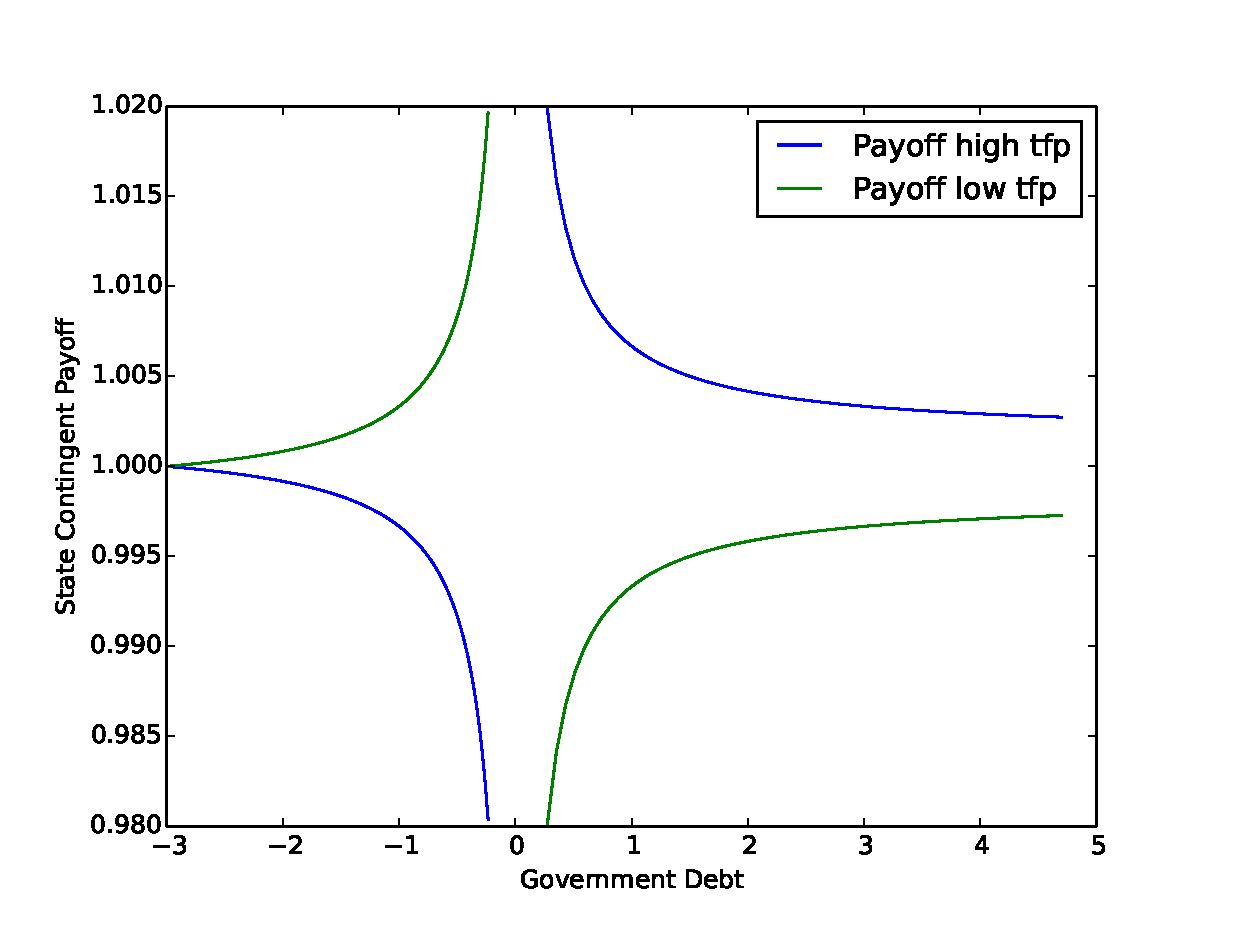
\includegraphics[scale=.4]{Images/p_graph_tfp.eps}
		\caption{Optimal asset payoff structure as a function of initial government debt when TFP follows a 2 shock i.i.d process}
	\end{center}	
	\end{figure}

  \end{frame}

%
  \begin{frame}
   \frametitle{Optimal Payoff Structure: Expenditure shocks}
	\begin{figure}
		\begin{center}
		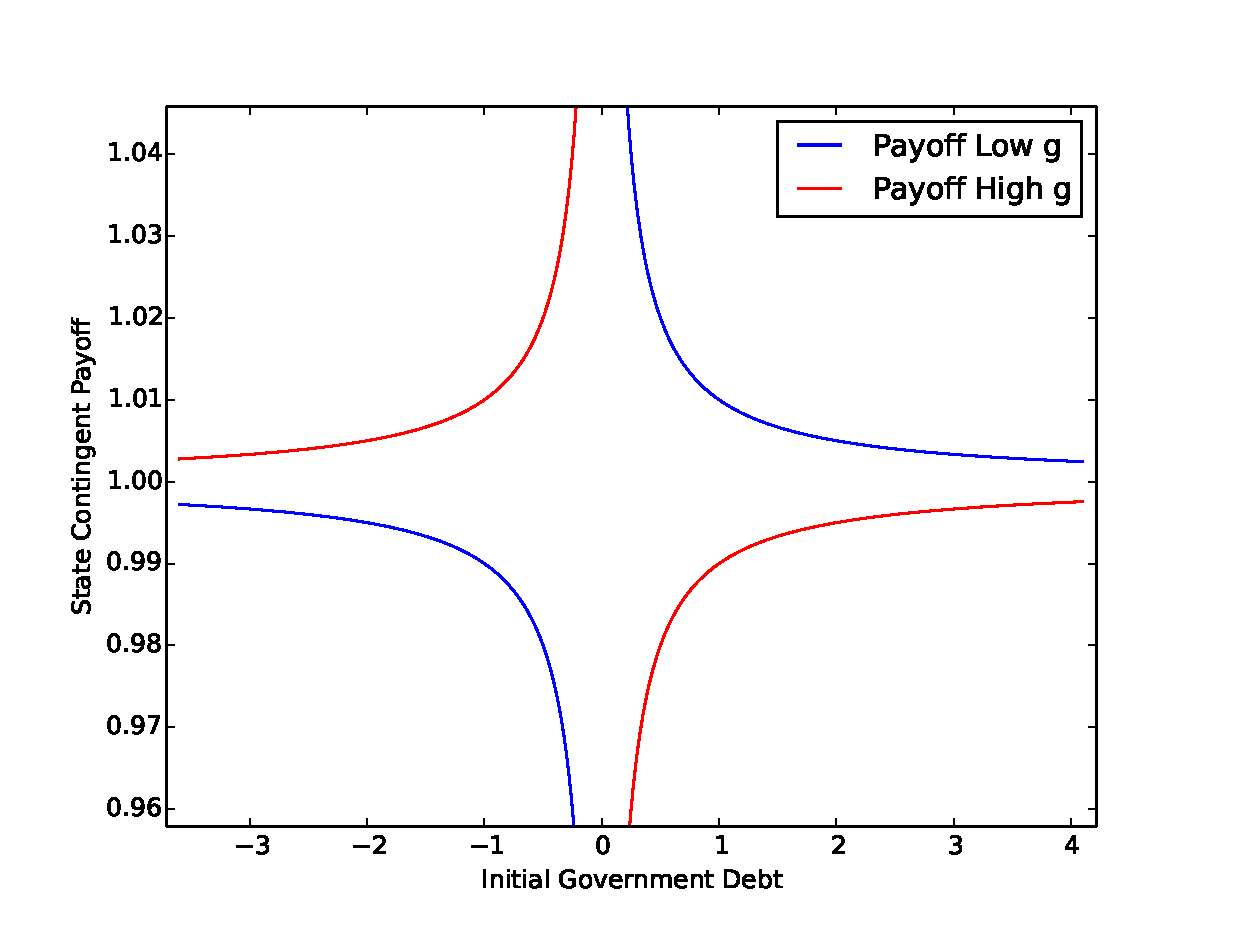
\includegraphics[scale=.4]{Images/p_graph.eps}
		\caption{Optimal asset payoff structure as a function of initial government debt when government expenditures follow 2 shock i.i.d process}
	\end{center}	
	\end{figure}

  \end{frame}
%
%


%
\begin{frame}
	\frametitle{Inverting the $\mathbb{P}^*$ mapping}
	\begin{enumerate}
		\item  \textbf{Exogenous payoff structure:} Suppose $\mathbb{P}\neq \mathbb{P}^*(b_{-1})$
		
		\item \textbf{Steady States: } A steady state is a government debt   $b^*$ such that
		\[b_{t}=b^* \text{ implies } b_{t+\tau}=b^*\quad \forall \tau >0\]
	
			
		\item \textbf{Characterization: } Given an asset payoff structure $\mathbb{P}$
		\begin{itemize}
			\item Does a steady state exist? Is it unique?
			\item Value of $b^*$?
			\item For what   \emph{initial government debts} $b_{-1}$ does  $b_t$ converge to $b^*$?
 			\end{itemize}
	\end{enumerate}
\end{frame}



 \begin{frame}
  \frametitle{Existence and $\mathbb{P}^{* -1}$}


 When shocks are i.i.d and take two values

  \begin{enumerate}

\item $\mathbb{P}(s|s\_)$ is independent of $s\_$ (so $\mathbb{P}$ can be a vector)
\item Under the normalization of $q_t = \beta$ we have $\mathbb{E}\mathbb{P}(s)=1$.   Payoffs are then determined by a single scalar $\bm{p}$.
\begin{itemize}
 \item $\bm{p}$ is the payoff in the ``good'' state $s$
 \item A risk-free bond is a security for which $\bm{p}=1$
\end{itemize}

\item A steady state is obtained by inverting the optimal payoff mapping $p^*$
\begin{equation*}
\label{eq-ss}
b^* \ \textrm{satisfies} \  \bm{p}=\bm{p}^*(b^*) \ \textrm{or} \ p^{* -1}(p) = b^*
\end{equation*}

One equation in one unknown $b^*$
\end{enumerate}
\end{frame}



\begin{frame}
\frametitle{Existence regions in $\bm{p}$ space}

The payoff $\bm{p}$ in good state
$\in (0,\infty)$.

We can decompose a set of economies with different asset payoffs into 3 regions via thresholds $\alpha_2\geq\alpha_1\geq1$



  \begin{itemize}
   \item Low enough $\bm{p}(\leq \alpha_1$): government holds assets in steady state
   \item High enough $\bm{p} (\geq \alpha_2$): government  issues debt  in steady state
   \item Intermediate $\bm{p} (\alpha_1>\bm{p}>\alpha_2$): steady state does not exist
  \end{itemize}

 \end{frame}




\begin{frame}
 \frametitle{Thresholds: $\alpha_1 <\alpha_2$}
	%For either a pure TFP shock or a pure government expenditure shock,  we compute % $\alpha_1$ and $\alpha_2$ directly
	\begin{itemize}
		\item With only government expenditure shocks
		\[
			\alpha_1 = 1 \text{  and }  \alpha_2 = (1-\beta)\frac{\theta^\frac{\gamma}{1+\gamma}\left(\frac{1}{1+\gamma}\right)^\frac1\gamma\frac{\gamma}{1+\gamma}-g(s_1)}{\theta^\frac{\gamma}{1+\gamma}\left(\frac{1}{1+\gamma}\right)^\frac1\gamma\frac{\gamma}{1+\gamma}-\EE g} +\beta>1
		\]
		\item With only TFP shocks
		\[
			\alpha_1 = (1-\beta)\frac{\theta(s_1)^\frac{\gamma}{1+\gamma}}{\EE\theta^\frac{\gamma}{1+\gamma}}+\beta > 1
		\]and
		\[
		\alpha_2 = (1-\beta)\frac{\theta(s_1)^\frac{\gamma}{1+\gamma}\left(\frac{1}{1+\gamma}\right)^\frac1\gamma\frac{\gamma}{1+\gamma}-g}{\EE\theta^\frac{\gamma}{1+\gamma}\left(\frac{1}{1+\gamma}\right)^\frac1\gamma\frac{\gamma}{1+\gamma}-g}+\beta>\alpha_1
		\]
	\end{itemize}
 \end{frame}


\begin{frame}
   \frametitle{Existence regions in $\bm{p}$ space}
	\begin{figure}
		\begin{center}
		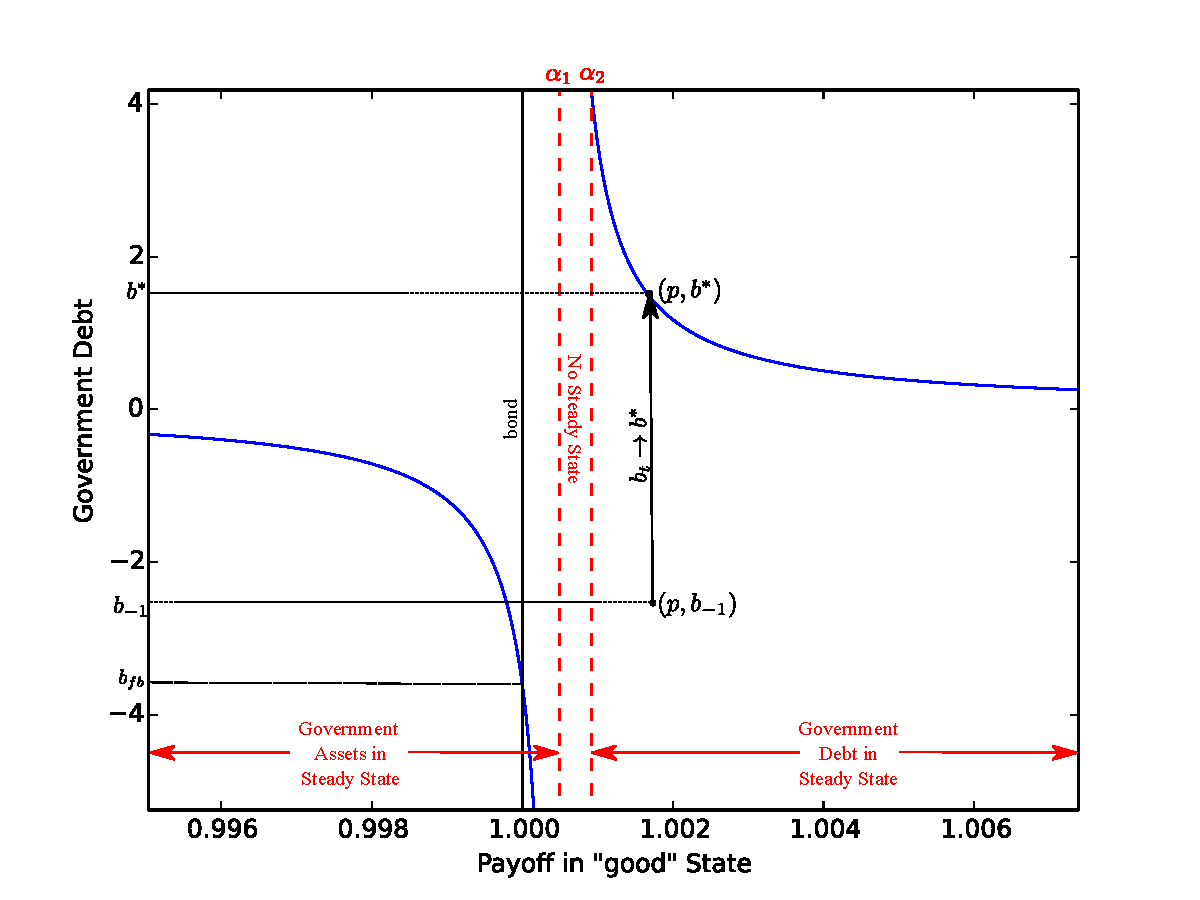
\includegraphics[width=4.2in]{Images/graph_nostable.pdf}
	\end{center}	
	\end{figure}

  \end{frame}


 \begin{frame}
  \frametitle{Convergence}
  \begin{itemize}
		\item Our analysis verifies existence of a steady state in a 2-state i.i.d. economy.
		\item To study long-run properties of a Ramsey allocation, we want to know whether steady state is stable
		\item \textbf{Risk-adjusted martingale:}
		
		The Lagrange multiplier $\mu_t$ on the implementability  constraint   satisfies
		\[
			\mu_t = \EE_t p_{t+1} \mu_{t+1}
		\] or
		\[
		\EE_t  \mu_{t+1}	= \mu_t -Cov_t (p_{t+1}, \mu_{t+1})
		\]
			%\emph{$\mu_t$ follows a risk adjusted martingale.}
	
		\item \textbf{Stability criterion: }   Away from a steady state, is the drift  of $\mu_t$ big enough?
		\end{itemize}
	

  \end{frame}

  \begin{frame}
  \frametitle{Characterizing convergence under quasi-linearity, iid, and $S=2$}

  \begin{itemize}
  \item Reminder:  $\bm{p}$ is the payoff in the ``good'' state.
   \item We partition  the ``$\bm{p}$ space'' into stable and unstable regions
     \end{itemize}

 	\begin{theorem}
Let $b^*$ denote steady state govt.  debt and $b_{fb}$ be  govt.  debt that  supports the first-best allocation with complete markets.  Then % for  same $  \alpha_1 < \alpha_2$
		\begin{enumerate}
			\item  \textbf{Low $\bm{p}$}: If $\bm{p}\leq\min(\alpha_1,1)$ then  $b_{fb}<b^*<0$ and $b_t\rightarrow b^*$ with probability 1.
			\item \textbf{High  $\bm{p}$}:  If $\bm{p} \geq \alpha_2$ then   $0<b^*$ and $b_t \rightarrow b^*$ with probability 1.
			
			
			\end{enumerate}
			\end{theorem}
			
			For the intermediate region where  $b^*$ either does not exist or is unstable, there is a tendency to run up debt
		
		
	
 \end{frame}


\begin{frame}
   \frametitle{Stability regions}
	\begin{figure}
		\begin{center}
		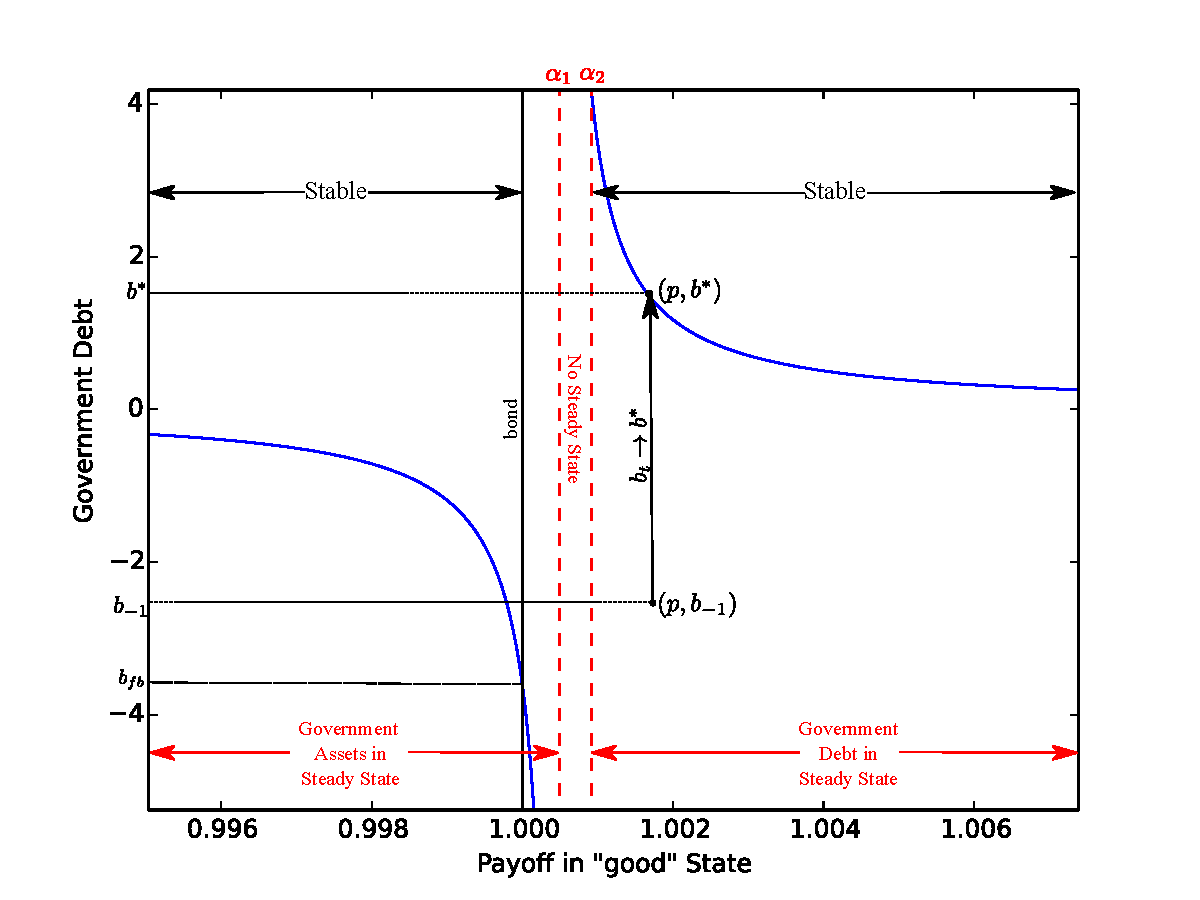
\includegraphics[width = 4.2in]{Images/graph_stable.pdf}
	\end{center}	
	\end{figure}

  \end{frame}


 \begin{frame}

	\frametitle{A sample path with  $\bm{p} > 1$}
	\begin{center}
	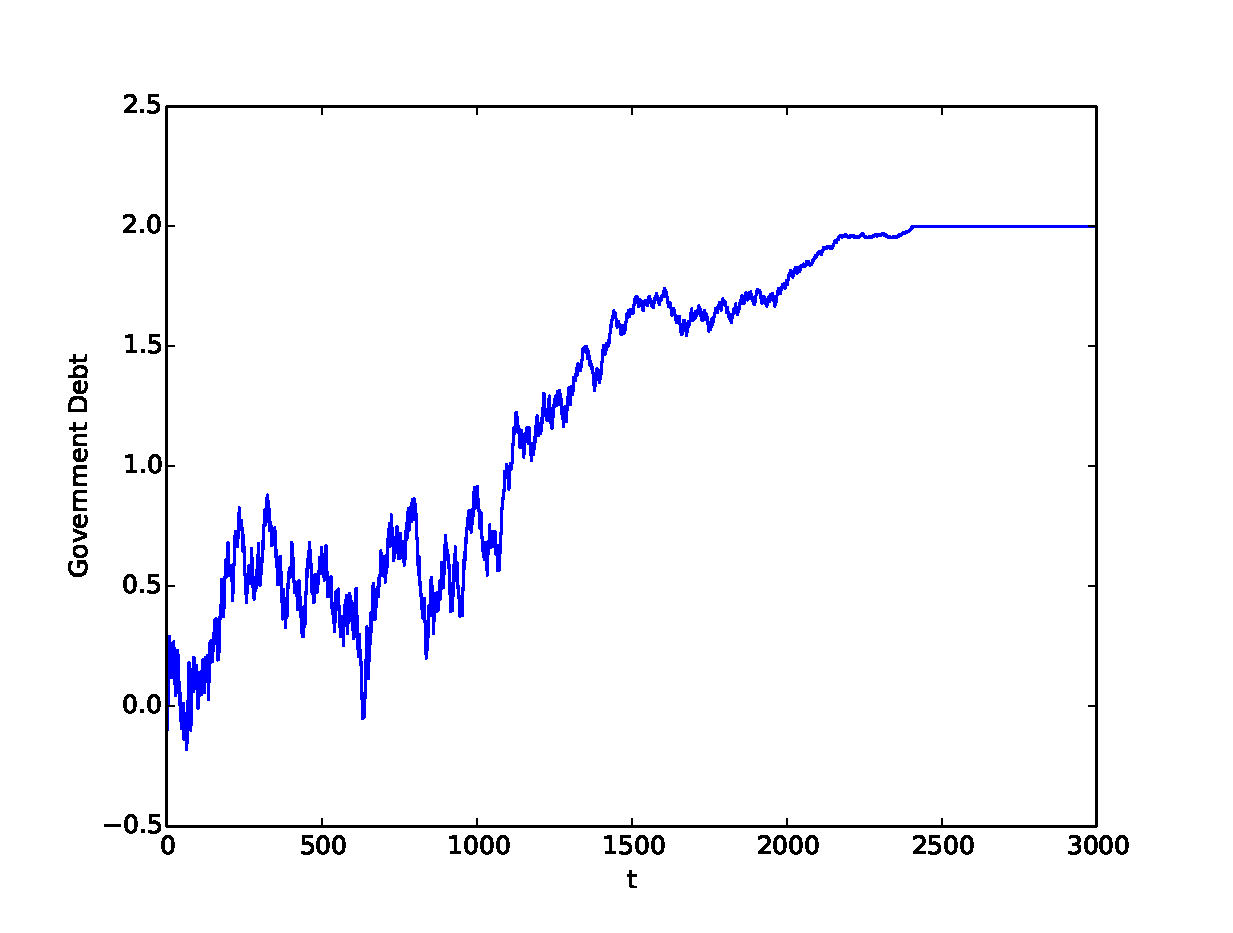
\includegraphics[width=4in]{Images/port1.eps}
	\end{center}
\end{frame}

\begin{frame}
	\frametitle{A sample path with   $\bm{p} <1$}
	\begin{center}
	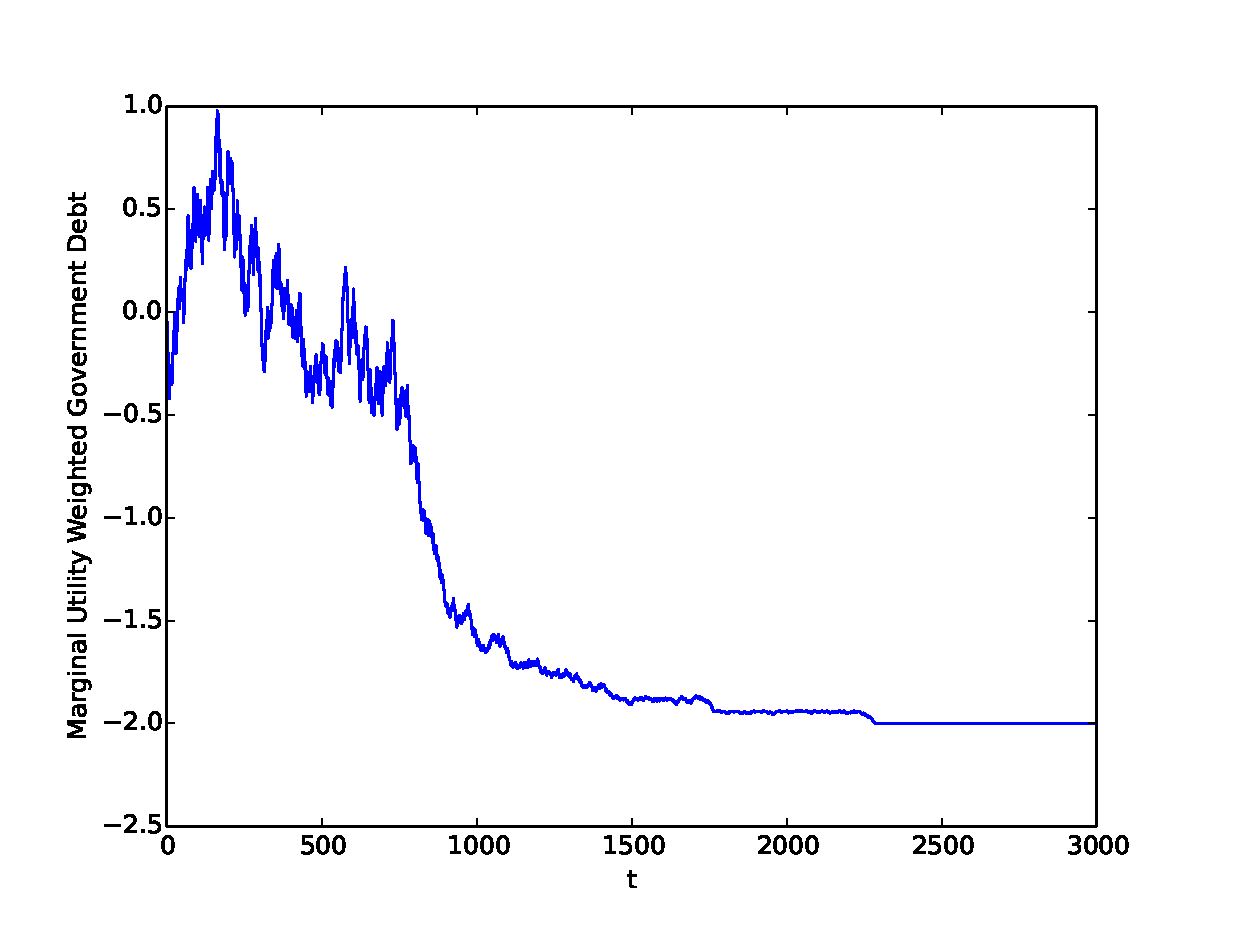
\includegraphics[width=4in]{Images/port2.eps}
	\end{center}
\end{frame}
%
% \begin{frame}
% 	\frametitle{Intuition and Generalizations}
% 	\begin{enumerate}
% 		\item The intuition we gain from our 2-state example is that, given exogenous payoff restrictions on government debt, there exist debt positions that allow the government to better smooth tax distortions across states.
% 		\item  Over time, the government adjusts it's debt position in order to best reallocate resources across states.
% 		\item  \textbf{Extensions: } more general preferences and more general aggregate state processes.
% 		\begin{itemize}
%
% 		\item  With risk aversion we are able to obtain similar results under the 2 state i.i.d assumption.
% 		\item More general processes require us to develop computational tools to analyze the long run dynamics
% 		\end{itemize}
%
% 		%\item  For more general aggregate state processes there no longer exists a complete markets %steady state.
% 		%\item  This requires us to develop computational tools to analyze the long-run dynamics.
% 		%\item  We find that with more general processes there exist regions with low volatility, because the government's debt position is reallocating resources across states and in the long run the government debt converges to these regions.
% 	\end{enumerate}
% \end{frame}
% %

\begin{frame}
	\frametitle{Intuition for Convergence}
	\small
	\begin{itemize}
	%\begin{itemize}
	%\item Debt {\color{black} \textbf{levels} } can help smooth tax distortions {\color{black}\textbf{across  states}}
	%\item This differs from the  role of debt economies with risk free debt where {\color{black} \textbf{changes}} in debt levels help smooth tax distortions {\color{black}  \textbf{over  time}}
	%\end{itemize}
	\item The optimal policy with incomplete markets smooths the welfare costs of distorting labor taxes by manipulating debt positions
	\item With a risk free bond the marginal cost of raising funds $\mu_t$ follow a martingale. In such economies,  changes in debt levels help smooth tax distortions across time. 		
	\item  If the payoff matrix of the asset differs across states, then level of government debt smooths tax distortions across states by generating state contingent revenues.
	\item The steady state $b^*$ is a unique debt level that provides the exact ``state contingency'' to overcome the missing assets markets	
	\item  When issuing debt the government takes takes this benefit into account, distorting the martingale, and leading to either the accumulation or decumulation of debt.	
	\item Although this is achived by raising taxes, locally,  the welfare costs of taxes is second order dominated by the gains from coming closer to $b^*$ which are first order in terms of welfare.
	\item This explains the long run convergence to $b^*$
	\end{itemize}
\end{frame}

\begin{frame}
 \frametitle{Outcomes with quasi-linear preferences}
 \textbf{Outcomes:}
 \begin{enumerate}
  \item  Often $b_t\to b^*$ when the aggregate state follows a 2-state i.i.d. process
  \item The level  and sign of $b^*$ depend on the \textbf{exogenous payoff structure} $\mathbb{P}$
  \item The limiting allocation corresponds to a complete market Ramsey allocation for initial govt. debt $b^*$
 \end{enumerate}

 \end{frame}



 \begin{frame}{Turning on risk-aversion}
  \textbf{Modifications:}
  \begin{itemize}
  \item Another source of return fluctuations -- the risk-free interest rate
   \item Marginal utility adjusted debt  encodes history dependence
   \item  With binary i.i.d shock shock process,  $x_t=u_{c,t}b_{t}$  converges

   \item Long-run properties of $x_t$ depend on equilibrium returns $R_{t,t+1}=\frac{\mathbb{P}(s_{t+1}|s_t)}{q_t(s^t)}$.
   Now $q_t$ varies in interesting ways


  \end{itemize}
  %\emph{To retain analytical tractability and clarify our analysis we will remove exogenous fluctuations in the payoff terms by restricting $p(s) =1$}
  \end{frame}
%


\begin{frame}
\frametitle{Roadmap, II}


 Two subproblems
\begin{enumerate}
 \item  $t=0$ Bellman equation in value function $W(b_{-1},s_0)$ %\textcolor{red}{Anmol and David XXXXXX: I altered the notation}
 \item  $t\geq 1$ Bellman equation in value function $V(x,s\_)$
\end{enumerate}

Seek steady states $x^*$ such that $x_t \to x^*$

\end{frame}




 \begin{frame}
	\frametitle{A Recursive Formulation}
	
	\begin{enumerate}
	 \item Commitment implies that government actions at $t \geq 1$ are constrained by the public's anticipations about them at $s < t$
	 \item This contributes additional state variables like marginal utility of consumption
	 \item Scaling the budget constraint by marginal utility makes Ramsey problem  recursive in  $x=U_c b$
	
	\[
		\frac{x_{t-1} p_t U_{c,t}}{\beta \EE_{t-1} p_t U_{c,t}}  = U_{c,t}c_t+U_{l,t} l_t + x_t
	\]
	
	%\item The planner's problem recursively with a single state variable.
	\end{enumerate}
	
	
	\end{frame}
	\begin{frame}
	\frametitle{Bellman equation for $t\geq1$ (\textit{ex ante})}
	\[
		V(x,s\_) = \max_{c(s),l(s),x'(s)} \sum_s \Pi(s,s\_)\Bigl(U(c(s),l(s)) + \beta V(x'(s),s)\Bigr)
	\]subject to $x'(s)\in [\underline x,\overline x]$
	\begin{align*}
		\frac{x \mathbb{P}(s) U_c(s)}{\beta\EE_{s\_} \mathbb{P}Uc} =U_c(s)c(s)+U_l(s)l(s) + x'(s)\\
		c(s) + g(s) = \theta(s)l(s)
	\end{align*}
	
 \end{frame}
\begin{frame}
	\frametitle{Time $0$ Bellman equation (\textit{ex post})}
	Given an initial  debt $b_{-1}$, state $s_0$,  and continuation value function $V(x,s\_)$
%\textcolor{red}{Anmol and David XXXXX: I altered the below by adding the $W$ function; but there is a problem with the timing of
%the $b$ argument.  See earlier slide where $W$ is defined.}
	\[
		W(b_{-1},s_0) = \max_{c_{0},l_0,x_{0}} U(c,l) +\beta V(x_0,s0)
	\]subject to  time zero implementability constraint
	\[
		U_{c}(c_0,l_0)c + U_l(c_0,l_0) l_0 + x_0 = U_c(c_0,l_0) b_{-1}
	\]and  resource constraint
	\[
		c_0+ g(s_0) = \theta(s_0) l_0
	\]and
	\[
		x_0 \in [\underline x,\overline x]
	\]
\end{frame}



\begin{frame}{Progress report}

\begin{enumerate}
 \item  Existence proved only under a special case of a risk-free bond  $\mathbb{P}(s|s\_)=1 \ \forall \ (s,s\_)$

 This focuses attention  on \textit{endogenous} component of returns coming from $q_t(s^t)$

 \item   $x^*$  is an initial condition for which the optimal asset payoff  in a LS economy is a risk-free bond

\end{enumerate}

\end{frame}

\begin{frame}
 \frametitle{Revisiting steady states with risk aversion}
Let $x'\left( s;{x},s\_\right) $ be an optimal  law of motion for the state variable
for the $t\geq1$ recursive problem.

\begin{definition}
 A steady state  ${x}^{*} $  satisfies ${ x}^{*}  =x' \left( s;{x}^{*},s_{-}\right) $ for all $%
\,s,s\_$
\end{definition}


\vspace{3mm}
\emph{Thus, a steady state is a node at which  continuation allocation and tax rate have no further history dependence. }

 \end{frame}




 \begin{frame}
	\frametitle{Existence}
	
	\begin{enumerate}
	 \item For a class of economies with separable iso-elastic preferences
	 $U(c,l) = \frac{c^{1-\sigma}}{1-\sigma} -\frac{ l^{1+\gamma}}{1+\gamma}$
	 \item Shocks that take two values and are i.i.d with $s_b$  being the ``adverse'' state (either low TFP or high expenditure)
	\end{enumerate}

	
	Let $x_{fb}$ be a value of the state $x$ from which a government can implement first=best with complete markets
	
	
	
	
	\begin{proposition}  Let $q_{fb}(s)$ be the shadow price of government debt in state $s$ using the first best allocation.
	If
	\[
		\frac{1-q_{fb}(s_b)}{1-q_{fb}(s_g)} > \frac{g(s_b)}{g(s_g)}>1
	\]
	
	Then there exists a steady state with $x_{fb}>x^*>0$
		\end{proposition}
\end{frame}


%



%
%
%
% \begin{frame}
% 	\frametitle{A Recursive Approach: Time 0}
% 	Given the initial debt level $b_0$, state $s_0$,  and the continuation value function $V(x,s\_)$ the planner's problem is then to solve the following
% 	\[
% 		\max_{c,l,x'} U(c,l) +\beta V(x',s0)
% 	\]subject to the time zero implementability constraint
% 	\[
% 		U_{c}(c,l)c + U_l(c,l) l + x' \geq U_c(c,l) b_0
% 	\]and the resource constraint
% 	\[
% 		c+ g(s_0) = \theta l
% 	\]and
% 	\[
% 		x' \in [\underline x,\overline x]
% 	\]
% \end{frame}
%
%
% %
% %   \item With risk aversion
% %   \item  To clarify our analysis we will remove exogenous fluctuations in the payoff terms $p_t U_{c,t}$ by restricting $p_t =1$.
% %  \end{enumerate}
% %
% % 	      \item quasilinear analysis found that there existed steady states when the aggregate state followed a 2 -state i.i.d. process.
% % 		\item Marginal utility weighted debt $x_t b_t U_{c,t}$ indexes the the space of optimal allocations with state contingent debt
% % 		\item  We would therefore expect a steady states to exist for the variable $x$
% % 		\item  To clarify our analysis we will remove exogenous fluctuations in the payoff terms $p_t U_{c,t}$ by restricting $p_t =1$.
% % 		\begin{itemize}
% % 			\item  Note under this restriction the endogenous payoff terms will be larger in bad states of the world, and thus, the government will hold assets in the steady state
% % 		\end{itemize}
% % 	\end{itemize}
% %\end{frame}
%
%
% \begin{frame}
% 	\frametitle{Incomplete Market's with Risk Aversion}
% 	\begin{itemize}
% 	\item By choosing a new variable $x_{t-1} = b_{t-1} U_{c,t-1}$ the measurability constraints can be written as a period by period constraint
% 	\[
% 		\frac{x_{t-1} p_t U_{c,t}}{\beta \EE_{t-1} p_t U_{c,t}}  = U_{c,t}c_t+U_{l,t} l_t + x_t
% 	\]
% 	\item  This bares a striking resemblance to the period by period constraint for quasi-linear preferences
% 	\[
% 		\frac{b_{t-1} p_t}{\beta \EE_{t-1} p_t} = c_t + U_{l,t} l_t + b_t
% 	\]
% 	\item  The $p_tU_{c,t}$ terms in the risk averse budget constraint act as endogenous payoffs.
% 	\end{itemize}
% \end{frame}
%
%  \begin{frame}
% 	\frametitle{Existence}
% 	Let $x_{fb}$ be the $x$ with which the government can institute first best from that period onwards.  Assume a CRRA utility specification $U(c,l) = \frac{c^{1-\sigma}}{1-\sigma} -\frac{ l^{1+\gamma}}{1+\gamma}$.  Finally, let  $c_{fb}$ and $l_{fb}$ be consumption and leisure under first best.  We have the following proposition
% 	\begin{proposition}  For a 2 state i.i.d. process let  $s_g$ and $s_b$ denoting the states with high and low consumption at first best.  If
% 	\[
% 		\frac{g(s_g)}{1-\frac{\beta\EE[(c_{fb})^{-\sigma}]}{c_{fb}(s_g)}} > \frac{g(s_b)}{1-\frac{\beta\EE[(c_{fb})^{-\sigma}]}{c_{fb}(s_b)}}
% 	\]  Then there exists a multiplier $\mu$ and complete markets solutions $c^\mu,l^\mu$ such that
% 	\[
% 	\underline x<\frac{U_{c_\mu}(s)c_\mu(s) + U_{l_\mu}(s) l_\mu(s)}{\frac{U_{c_\mu}(s)}{\beta\EE[U_{c_\mu}]}-1} = x^* <0
% 	\]
% 	\end{proposition}
% \end{frame}
%
%
\begin{frame}
	\frametitle{Stability}
	\begin{enumerate}
	 \item Here interest rates are aligned with marginal utility of consumption;  they are low  in ``good'' states (high TFP or low expenditure)
	 \item The government holds claims against the private sector in the steady state. Similar to the quasilinear case with  low  $\bm{p}$	
	 \item The incomplete markets Ramsey allocation converges to a Lucas-Stokey  Ramsey allocation for all initial conditions	 	
	\end{enumerate}


	\begin{proposition}  Let $\{c_t(s^t), l_t(s^t), x_t(s^{t-1})\}$ solve the incomplete markets Ramsey problem with $x_0 > x^*$.  Then  $x_t(s^{t-1})\rightarrow x^*$ as $t\rightarrow \infty$ with probability 1 for all initial conditions
	
	\end{proposition}
	\end{frame}
	
%
% \begin{frame}
% 	\frametitle{Quasilinear vs. risk aversion}
% 	{\color{red} Redo this slide}
% 	\begin{itemize}
% 				\item  With  quasilinear preferences and a risk-free bond, the interest rate is always $1/\beta$.
%    \item With risk averse preferences, interest rate is higher in periods of high government expenditure.
% 		\item  Thus, while the government has greater expenses in high government expenditure states, the higher interest rate means that the government can  accumulate less and still  cover future government expenditures.
% 		\item  After the government has accumulated enough assets, it is actually better off in periods of high government expenditure than in periods with low government expenditures (since its claims to consumption are worth more).
% 		\item  By holding assets, the government is able to reallocate resources across states, something it is not able to do in the quasilinear case.
% 	\end{itemize}
% \end{frame}
%
\begin{frame}
	\frametitle{A sample path for 2 state i.i.d. process with risk aversion}
	\begin{center}
	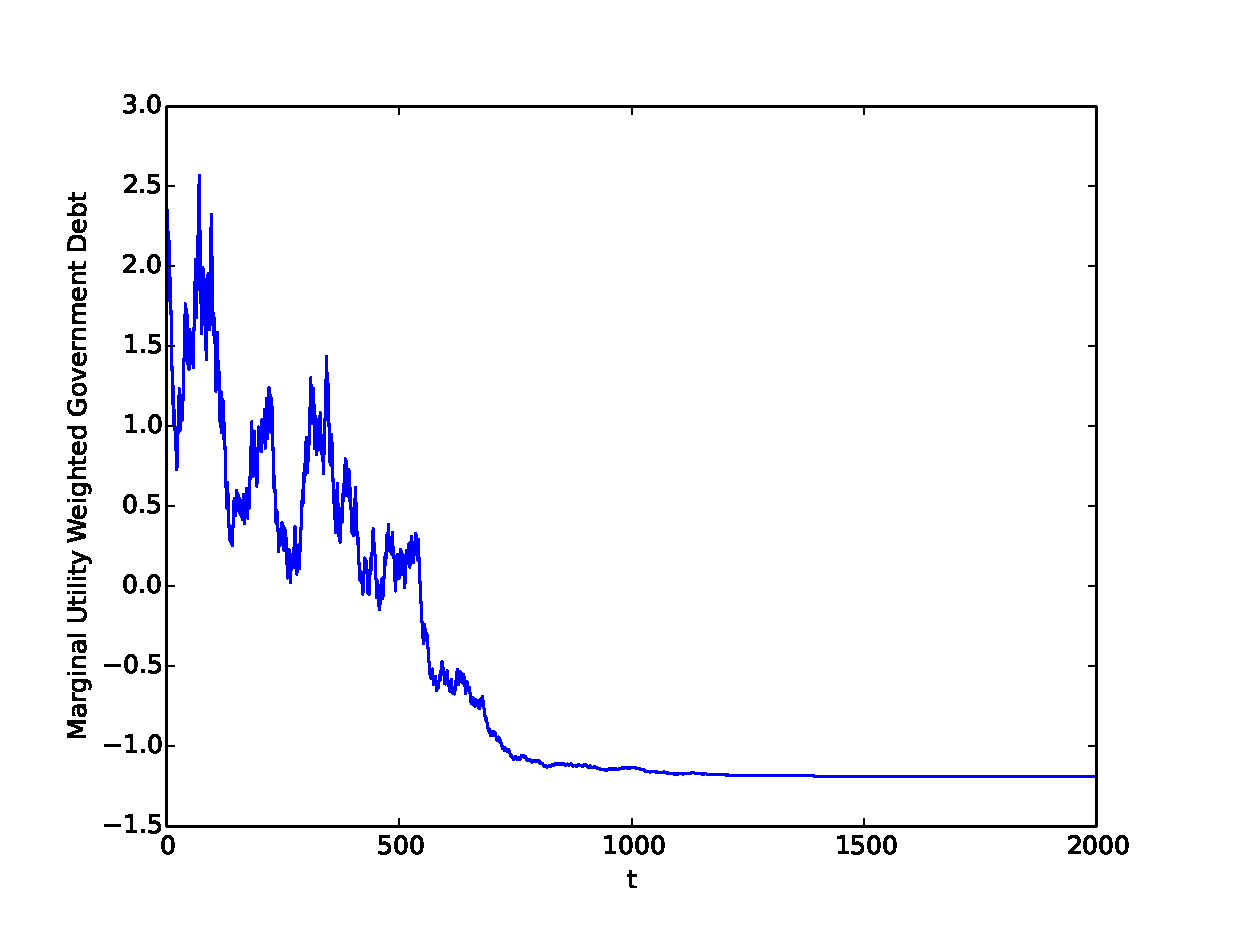
\includegraphics[width=4in]{Images/2stateiid.eps}
	\end{center}
\end{frame}

\section{Numerical Results}
\subsection{}

\begin{frame}
	\frametitle{A sample path  for economy with $S>2$ states}
	\begin{center}
	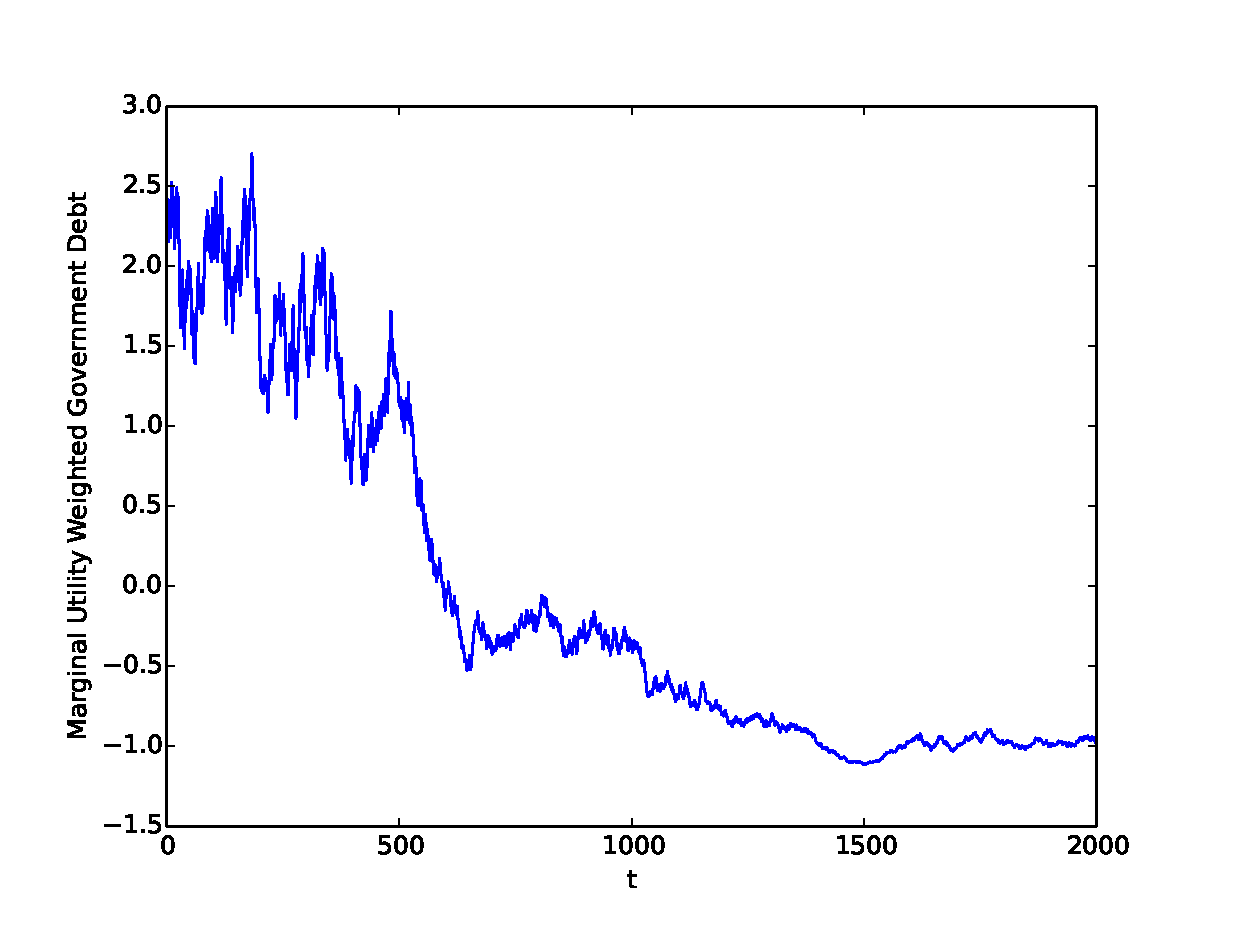
\includegraphics[width=4in]{Images/5stateiid.eps}
	\end{center}
\end{frame}



 \begin{frame}
  \frametitle{Transfers}
	\begin{itemize}	
	\item Access to nonnegative transfers makes first-best level of assets trivially a ``steady state''  	
\item  All results hold \textit{on one side} of steady state
\begin{theorem}

With nonnegative lump sum transfers,  in cases where a steady state exists and is stable,  if the initial debt of the government exceeds its steady state level,  the economy  converges with probability 1 to the steady state.

\end{theorem}
		
	\end{itemize}
 \end{frame}

 \begin{frame}
	\frametitle{Quasilinear preferences and risk-free bond  with and without nonnegative transfers}
	\begin{center}
	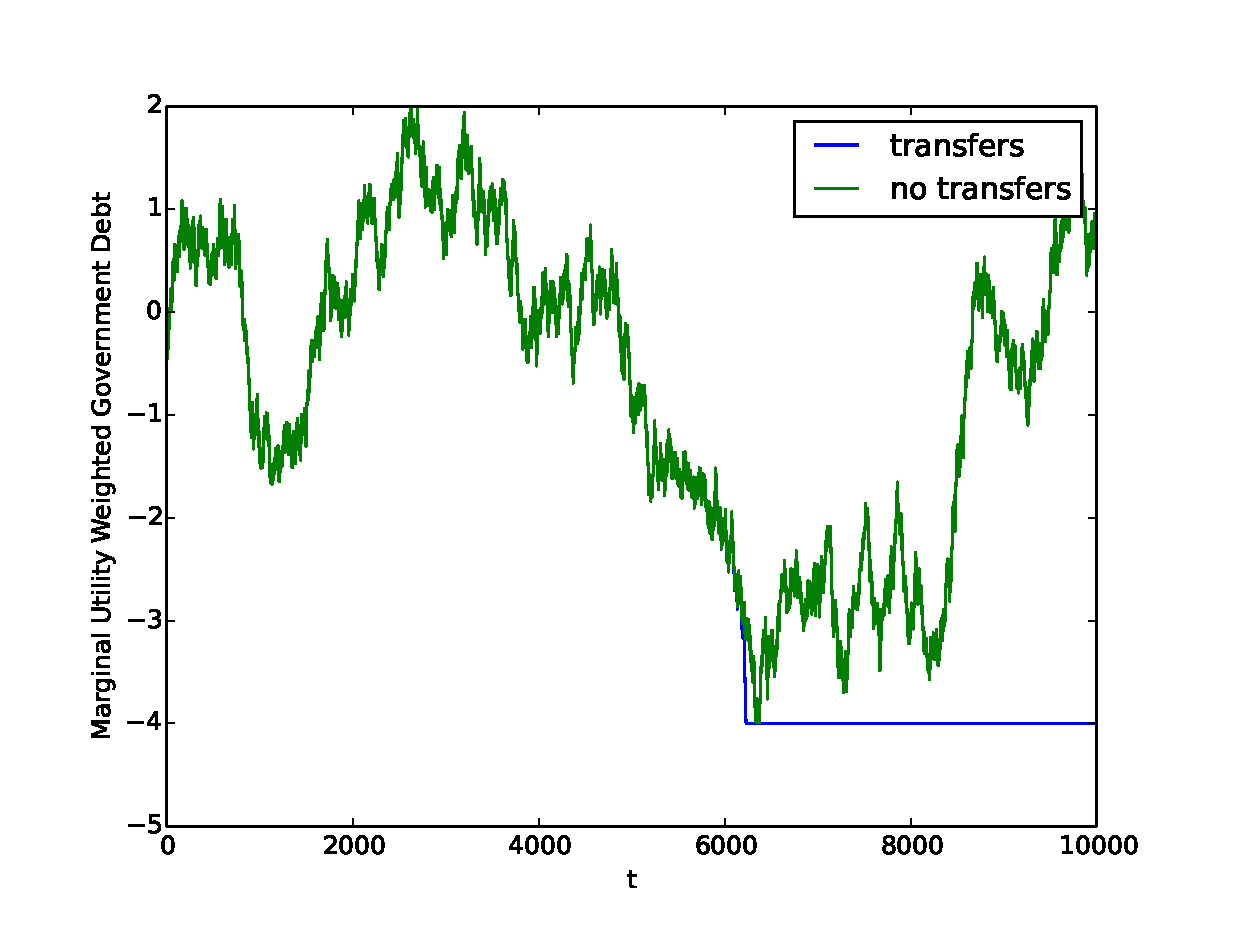
\includegraphics[width=4in]{Images/transfer_example2.eps}
	\end{center}
\end{frame}


%\begin{frame}{Battle field}
%\small
%\textit{What are the long run levels of government holdings ?}
%
%\vspace{3mm}
%
%With shocks that are IID and take two values,
%
%\begin{tabular}[h]{| l | p{1.25in} | p{1.25in} |}
%	\hline
%	&$p = 1$& $p\neq 1$\\
%	\hline
%	Quasi-Linear& (AMSS)
%	
%	With $T_t\geq 0$, hold assets at first best .&Partition the payoff space such that either
%	
%	a) issue or
%	b) run up debt eventually\\
%	\hline
%	Risk Aversion& Conditions under which
%	
%	assets $<$ first best& \emph{Conjecture:} Similar results  as in quasi-linear case\\
%	\hline
%\end{tabular}
%
%
%\vspace{4mm}
%
%In future work we plan to study more general shocks processes
%
%\end{frame}
\begin{frame}{Battlefield}
\small
\textit{What is government debt in long-run?}


\vspace{3mm}

With shocks that are IID and take two values

\medskip


\begin{tabular}[h]{| l | p{1.25in} | p{1.25in} |}
	\hline
	&risk-free bond & risky bond \\
	\hline
	Quasi-Linear& (AMSS)
	
	With $T_t\geq 0$, govt. accumulates enough assets for first best.&Partition  payoff space so that govt. either
	
	a) issues or
	b) runs up debt eventually\\
	\hline
	Risk Aversion& Conditions under which limiting govt.	
	assets $<$ first best& \emph{Conjecture:} Similar to quasi-linear outcomes\\
	\hline
\end{tabular}


\vspace{4mm}

In future work we plan to study more general shocks processes

\end{frame}


\begin{frame}
 \frametitle{Comparison to literature}
 \begin{enumerate}
  \item Angelotos (2002), Buera and Nicolini (2004)

\begin{itemize}
 \item Begin with a complete market  Ramsey allocation
 \item Ask if this can be spanned by \emph{some} collection of non-contingents debt of different maturities?
\end{itemize}
\item This paper
\begin{itemize}
 \item Begin with an incomplete markets Ramsey allocation
 \item Ask whether the long-run allocation coincides with \emph{some} complete market allocation?
\end{itemize}

\item In BEGS1, we study a related problem with heterogeneous agents




 \end{enumerate}


\end{frame}


\end{document}

 \begin{frame}
  \frametitle{Concluding remarks }
\begin{itemize}
	\item With market incompleteness, the asset payoff structure  has big implications a Ramsey government's  long run debt
	\item If the asset offers lower returns in adverse states of the world, the Ramsey government  asymptotically runs up a  debt to the private sector.
\item With risk aversion, cyclical properties of interest rate affects government debt asymptotically
	\item  Access to nonnegative transfers play little role in shaping outcomes.  Rather, the key  force is the government's ability to use its debt position to reallocate resources across states
	\item  \textbf{Future Research}:   With heterogeneous agents and unrestricted transfers, how does the type of market incompleteness affect long run wealth distributions and other outcomes?
\end{itemize}
 \end{frame}

  \end{document}
=======
\documentclass{beamer}
\usetheme{default}
\setbeamertemplate{navigation symbols}{}
%	
\usepackage{subfig}
\usepackage{amsmath, amsthm, amssymb}
\usepackage{float}
\usepackage{rotating}
\usepackage{graphicx}
\usepackage{epstopdf}
\usepackage{longtable}
\usepackage{xcolor}
\usepackage{bm}
\usepackage{tikz}
\usetikzlibrary{shapes}
\tikzset{My Arrow Style/.style={single arrow, fill=red!50, anchor=base, align=center,text width=.5cm,rotate =270}}
\newcommand{\MyArrow}[2][]{\tikz[baseline] \node [My Arrow Style,#1] {#2};}
\tikzset{My 2Arrow Style/.style={single arrow, fill=red!50, anchor=base, align=center,text width=.5cm,rotate =90}}
\newcommand{\MyArrowUp}[2][]{\tikz[baseline] \node [My 2Arrow Style,#1] {#2};}
%\newcommand{at}{\begin{matrix}}
%\newcommand{\emat}{\end{matrix}}
\newcommand{\EE}{\mathbb E}

\newtheorem{acknowledgement}[theorem]{Acknowledgement}
\newtheorem{algorithm}[theorem]{Algorithm}
\newtheorem{assumption}{Assumption}
\newtheorem{axiom}{Axiom}
\newtheorem{case}[theorem]{Case}
\newtheorem{claim}[theorem]{Claim}
\newtheorem{conclusion}[theorem]{Conclusion}
\newtheorem{condition}[theorem]{Condition}
\newtheorem{conjecture}{Conjecture}
\newtheorem{criterion}[theorem]{Criterion}
\newtheorem{proposition}{Proposition}
\newtheorem{summary}[theorem]{Summary}
\newtheorem{exercise}{Exercise}
\newtheorem{notation}{Notation}
\newtheorem{remark}{Remark}
%\graphicspath{{graphs//}}

\title {Optimal Taxation Without State Contingent Debt}
\author{Anmol Bhandari, David Evans, Mikhail Golosov, Thomas J. Sargent}

\date{October 2013}
% \today will show current date.
% Alternatively, you can specify a date.
%
\begin{document}
%
\begin{frame}
\titlepage

\end{frame}
\section{Introduction}
\subsection{}
\begin{frame}
\frametitle{Commitment, representative agent, no capital}

\begin{itemize}

 \item \textbf{Incomplete markets}

 \quad \color{red}$\rightarrow$ \color{black} A single, possibly risky asset

 \item \textbf{Linear tax schedules}

 \quad \color{red}$\rightarrow$ \color{black}Proportional tax on labor earnings (maybe plus  {\em nonnegative} transfers)

 \item \textbf{Aggregate shocks}

 \quad \color{red}$\rightarrow$ \color{black} To productivities, government expenditures

 \end{itemize}
\end{frame}



\begin{frame}
\frametitle{Questions}

\begin{enumerate}
\item Should a  government accumulate or decumulate assets?
\item Why might different governments want to issue different amounts of debt?
\item Existing answers hinge on polar assumptions:
\begin{itemize}
 \item [+] Complete markets, Lucas Stokey (1984): non history dependent debt quantities inherited from initial condition
 \item [+ ] A risk-free bond only, quasi-linear preferences, AMSS (2002): govt. accumulates {\em assets} sufficient to finance activities using interest revenues
\end{itemize}
\item Unknown: what if interest rates fluctuate?
\end{enumerate}
\end{frame}

%
%\begin{frame}
%\frametitle{Our analysis}
%
%\begin{enumerate}
%\item \textbf{Asset structure}
%\begin{itemize}
%\item [+] A single asset only
%\item [+] We exogenously restrict asset payoffs
%
%% $\Longrightarrow$ E.g., bonds that pay less during adverse times
%
% \end{itemize}
%\item \textbf{Economic forces}
%\begin{itemize}
%\item Asset {\color{black} \textbf{levels} } can help smooth tax distortions {\color{black} \textbf{ across  states}}
%\item This differs from the  role of debt in previous incomplete markets  economies where { \color{black} \textbf{changes}} in debt levels help smooth tax distortions {\color{black}  \textbf{ over  time}}
%\end{itemize}
%\end{enumerate}
%
%\end{frame}


\section{Environment}
\subsection{}

\begin{frame}
 \frametitle{Environment}
 \begin{itemize}
 \item \textbf{Uncertainty}: Markov aggregate shocks $s_t\in \mathcal{S}$; $S \times S$ stochastic matrix $\Pi$
  \item \textbf{Demography}: Infinitely lived representative agent plus a benevolent planner
  \item \textbf{Preferences }(representative household)
  \begin{equation*}
\mathbb{E}_{0}\sum_{t=0}^{\infty } \beta^t  U\left(
c(s^t),l(s^t)\right)  \label{utility lifetime}
\end{equation*}%
  \item \textbf{Technology}: Aggregate output  $y_t=\theta_{t} l_{t}$
   \end{itemize}

\end{frame}

\begin{frame}
 \frametitle{Environment, II}
 \begin{itemize}
\item \textbf{Asset market}:
\begin{itemize}
 %\item A single asset
\item $S \times S$ matrix $\mathbb{P}$ with time $t$ payoff being
\[p_t=\mathbb{P}(s_{t}|s_{t-1})\]
\end{itemize}



  \item \textbf{Linear Taxes}: Agent $i$'s tax bill
\[- T_t + \tau_t \theta_{t}l_{t},  \ T_t \geq 0 \]

\item[]
  \item \textbf{Budget constraints} $q_t$ is price of  asset

  \begin{itemize}
   \item Household: $ c_{t}+q_tb_{t}=\left( 1-\tau _{t}\right) \theta _{t}l_{t}+p_{t}b_{t-1}+T_{t}$ % \ T_t \geq 0$
  \item Government: $g_{t}+q_tB_{t}+T_t=\tau _{t}\theta_{t}l_{t}+p_{t}B_{t-1} $% \ T_t \geq 0$
  \end{itemize}

\item[]
  \item \textbf{Market Clearing}
  \begin{itemize}
   \item Goods: $c_{t}+g_t = \theta _{t} l_{t}$

   \item Assets: $b_{t}+B_{t}=0$
\end{itemize}
  \item[]

\item \textbf{Initial conditions}: Assets $b_{-1}, B_{-1}$ and  $s_{-1}$
\end{itemize}

\end{frame}

\begin{frame}
 \frametitle{Ramsey Problem}

\begin{definition}
\textbf{Allocation, price system, government policy}

\end{definition}

\begin{definition}
\textbf{Competitive equilibrium}: Given $\left(b_{-1},B_{-1},s_{-1}\right) $ and $\left\{ \tau _{t},T_{t}\right\} _{t=0}^{\infty }$,
all allocations are individually rational, markets clear \footnote{Usually, we impose only  ``natural'' debt limits. }
\end{definition}

\begin{definition}
\textbf{Optimal competitive equilibrium}: A welfare-maximizing competitive
equilibrium for a given $\left( b_{-1},B_{-1},s_{-1}\right) $
\end{definition}

 \end{frame}

\begin{frame}
  \frametitle{Ramsey problem}

  \begin{enumerate}
  \item \textbf{Primal approach}: To eliminate tax rates and prices, use  household's first order conditions:
\begin{subequations}
	\[
		U_{c,t} q_t = \beta \EE_t U_{c,t+1}
	\]
	\[
		(1-\tau_t)\theta_tU_{c,t} = - U_{l,t}
	\]
\end{subequations}
  \item \textbf{Implementability constraints}:  Derive by iterating the household's budget equation forward  at every history

  $\Rightarrow$ for $t \geq 1$, these impose  \emph{measurability restrictions} on Ramsey allocations

\item The $t\geq 1$ \textbf{measurability constraints} contribute the only difference from Lucas-Stokey's Ramsey problem.

 \end{enumerate}




  \end{frame}



\begin{frame}
  \frametitle{Ramsey problem}

  \begin{enumerate}



  \item[4.]  \textbf{Transfers: } We temporarily restrict transfers $T_t = 0$  $\forall t$. This is convenient for our analytical results.  We eventually show  that this assumption is not restrictive.

\end{enumerate}



  \end{frame}




 \begin{frame}
 \frametitle{Ramsey problem (Lucas-Stokey)}
\begin{equation*}
\max_{\{c_t,l_t,b_t\}} \EE_0\sum_{t=0}^\infty \beta^t U(c_t,l_t)
 \end{equation*}
 subject to

 \vspace{3mm}

 (a) \textbf{Feasibility}
\begin{subequations}
\begin{equation*}
c_t + g_t = \theta_t l_t
 \end{equation*}

(b) \textbf{Implementability constraint}

% \begin{equation*}
% \frac{b_{t-1}U_{c,t-1}}{\beta} = \frac{\EE_{t-1} p_t U_{c,t}}{p_t U_{c,t}}\EE_t\sum_{j=0}^\infty\beta^j\left( U_{c,t+j}c_{t+j}+U_{l,t+j}l_{t+j}\right)\text{  for $t\geq 1$ }
% \end{equation*}
\begin{equation*}
b_{-1} = \frac1{U_{c,0}}\EE_0\sum_{t=0}^\infty \beta^t\left(U_{c,t}c_t+U_{l,t}l_t\right)
 \end{equation*}
\end{subequations}
  \end{frame}



 \begin{frame}
 \frametitle{Ramsey problem (BEGS)}
\begin{equation*}
\max_{\{c_t,l_t,b_t\}} \EE_0\sum_{t=0}^\infty \beta^t U(c_t,l_t)
 \end{equation*}

 \vspace{3mm}

 (a) \textbf{Feasibility}
\begin{subequations}
\begin{equation*}
c_t + g_t = \theta_t l_t
 \end{equation*}

(b) \textbf{Lucas-Stokey implementability constraint}
\begin{equation*}
b_{-1} = \frac1{U_{c,0}}\EE_0\sum_{t=0}^\infty \beta^t\left(U_{c,t}c_t+U_{l,t}l_t\right)
 \end{equation*}

 (c) \textbf{Measurability constraints}
 \begin{equation*}
 \frac{b_{t-1}U_{c,t-1}}{\beta} = \frac{\EE_{t-1} p_t U_{c,t}}{p_t U_{c,t}}\EE_t\sum_{j=0}^\infty\beta^j\left( U_{c,t+j}c_{t+j}+U_{l,t+j}l_{t+j}\right)\text{  for $t\geq 1$ }
 \end{equation*}
\end{subequations}
  \end{frame}


\begin{frame}
\frametitle{Roadmap, analytic strategy}

	\begin{itemize}
	\item Properties of a Ramsey allocation -- especially asymptotic ones --   vary with   \textbf{asset returns} that reflect
	\begin{itemize}
	 \item Prices $\{q_t(s^t|B_{-1},s_{-1})\}_t$
	 \item Payoffs $\mathbb{P}$
	\end{itemize}
	
\item To focus on the exogenous $\mathbb{P}$ part of return, we first study quasi-linear  preferences  that pin down $q_t=\beta \mathbb{E}_t
\mathbb{P}(s_{t+1}|s_t)$

\item Turn on  risk aversion and fluctuating $q_t$ later
	
\end{itemize}
\end{frame}



\begin{frame}{Battle field}

\textit{What is government debt in long-run?}

\vspace{3mm}


\bigskip
\begin{tabular}[h]{| l | p{1.25in} | p{1.25in} |}
	\hline
	&risk-free bond & risky bond \\
	\hline
	Quasi-Linear&  & \\
	\hline
	Risk Aversion & &  \\
	\hline
\end{tabular}


\vspace{4mm}



\end{frame}

\begin{frame}
\frametitle{Analysis with quasi-linear preferences}


Quasilinear preferences $U(c,l)=c-\frac{l^{1+\gamma}}{1+\gamma}$

 To characterize \textbf{long-run}  debt and  taxes,  we construct and then invert  mapping $\mathbb{P}^*(b)$

\begin{itemize}
 \item Given \textbf{arbitrary} initial govt. assets $b_{-1}$, what is  an \textbf{optimal} asset payoff matrix $\mathbb{P}^* =\mathbb{P}^*(b_{-1})$?

 \item Under a Ramsey plan for an \textbf{arbitrary} payoff matrix $\mathbb{P}$,  when would  $b_t \to b^*$, where

	\[\mathbb{P}=\mathbb{P}^*(b^*) \ \textrm{or} \ b^* = \mathbb{P}^{* -1}(\mathbb{P}) ?\]
	
\end{itemize}
\end{frame}

\begin{frame}
\frametitle{Roadmap, the answers}


	
	\begin{itemize}
	\item We first reverse engineer an optimal $\mathbb{P}^*(b_{-1})$ from a Lucas-Stokey  Ramsey allocation
	
	 \item In a binary IID world, we identify a big set of  $\mathbb{P}$'s that imply that $b_t$  under a Ramsey plan converges to $b^*$ that solves
	
	\[\mathbb{P}=\mathbb{P}^*(b^*)\]
	
	
	\item For more general shock structures, we numerically verify  an ergodic set of $b_t$'s
 hovering around $\tilde b$.    The optimal $\mathbb{P}^*$ associated with $\tilde b$ seems close to $\mathbb{P}$:
	\[\mathbb{P}\approx \mathbb{P}^*(\tilde b)\]
%	\textcolor{red}{Anmol and David XXXXXX: the preceding approximate equality needs clarification at least for me. What does it mean?}
	\end{itemize}

	
\end{frame}
%
% %
% %
% % \begin{frame}
% % \frametitle{Roadmap}
% % 	\begin{itemize}
% % 		\item  We will begin by characterizing the optimal payoff structure the government would choose if it did not have this exogenous restriction
% % 		\begin{itemize}
% % 			\item  This is done by directly solving for the optimal allocation with state contingent debt.
% % 		\end{itemize}
% % 		\item We wish to characterize the solution to the optimal planning problem when the payoff structure is not optimal.
% % 		\item  With general preferences the government asset returns have both exogenous components ($p_s$) and endogenous components (stochastic discount factor).
% % 		\item  We will initially restrict ourselves to the quasilinear case, in order to remove the endogenous component.
% % 	\end{itemize}
% % \end{frame}
% %
%
  \begin{frame}
\frametitle{Optimal asset payoff matrix $\mathbb{P}^*$}
\begin{enumerate}
 \item  Given $b_{-1}$, compute a Lucas-Stokey Ramsey allocation

% \emph{Find an  optimal allocation ignoring $t\geq 1$ measurability constraints.}

 \item Reverse engineer  payoff on single asset
\[
	p_t = \frac{\beta}{U_{c,t}b_{t-1}}\EE_t\sum_{j=0}^\infty\beta^j\left(U_{c,t+j}c_{t+j}+U_{l,t+j}l_{t+j}\right)
\]
\item By construction, the optimal payoff  $p_t$   disarms the  $t\geq 1$
measurability constraints
\item Since a Lucas-Stokey Ramsey allocation is  history independent,
\[p_t=\mathbb{P}^*(s_t|s_{t-1})\]
\end{enumerate}
\end{frame}
%
\begin{frame}
\frametitle{Quasilinear preferences $U(c,l)=c-\frac{l^{1+\gamma}}{1+\gamma}$}
Given
 initial assets $b_{-1}$,  let $\mu(b_{-1})$ be the Lagrange multiplier on the Lucas-Stokey implementability constraint
\begin{enumerate}

 \item \textbf{Multiplier $\to$ Tax rate:}
 \[
		\tau(\mu) = \frac{\gamma\mu}{(1+\gamma)\mu-1}
	\]
 \item \textbf{Tax rate $\to$ net of interest surplus:}
 \[
		S(s,\tau) = \theta(s)^\frac\gamma{1+\gamma}(1-\tau)^\frac1\gamma\tau-g(s)
	\]
\item \textbf{Surplus $\to$ optimal payoff structure:}

\[
 \mathbb{P}^*(s|s\_) = (1-\beta)\frac{S(s,\tau)}{\EE_{s\_} S(s,\tau)} + \beta
 \]

 \end{enumerate}

\end{frame}

%
% 		
\begin{frame}		
   \frametitle{Initial holdings influence optimal asset payoff structure}
Denote state $s$ as ``adverse''  if it has ``high'' govt. expenditures or ``low '' TFP; formally, $s$ is ``adverse'' if
\[   g(s)\EE_{s\_}\theta^\frac{\gamma}{1+\gamma}-\theta(s)^\frac\gamma{1+\gamma}\EE_{s\_} g >0\]

Properties of  optimal payoff matrix $\mathbb{P}$

\begin{itemize}
 \item With positive initial govt. assets: want an asset  that pays {\em more} in ``adverse'' states
 \item With negative initial govt. assets: want an asset  that pays {\em less} in ``adverse'' states
\end{itemize}
\end{frame}


  \begin{frame}
   \frametitle{Optimal Payoff Structure: TFP shocks}
	\begin{figure}
		\begin{center}
		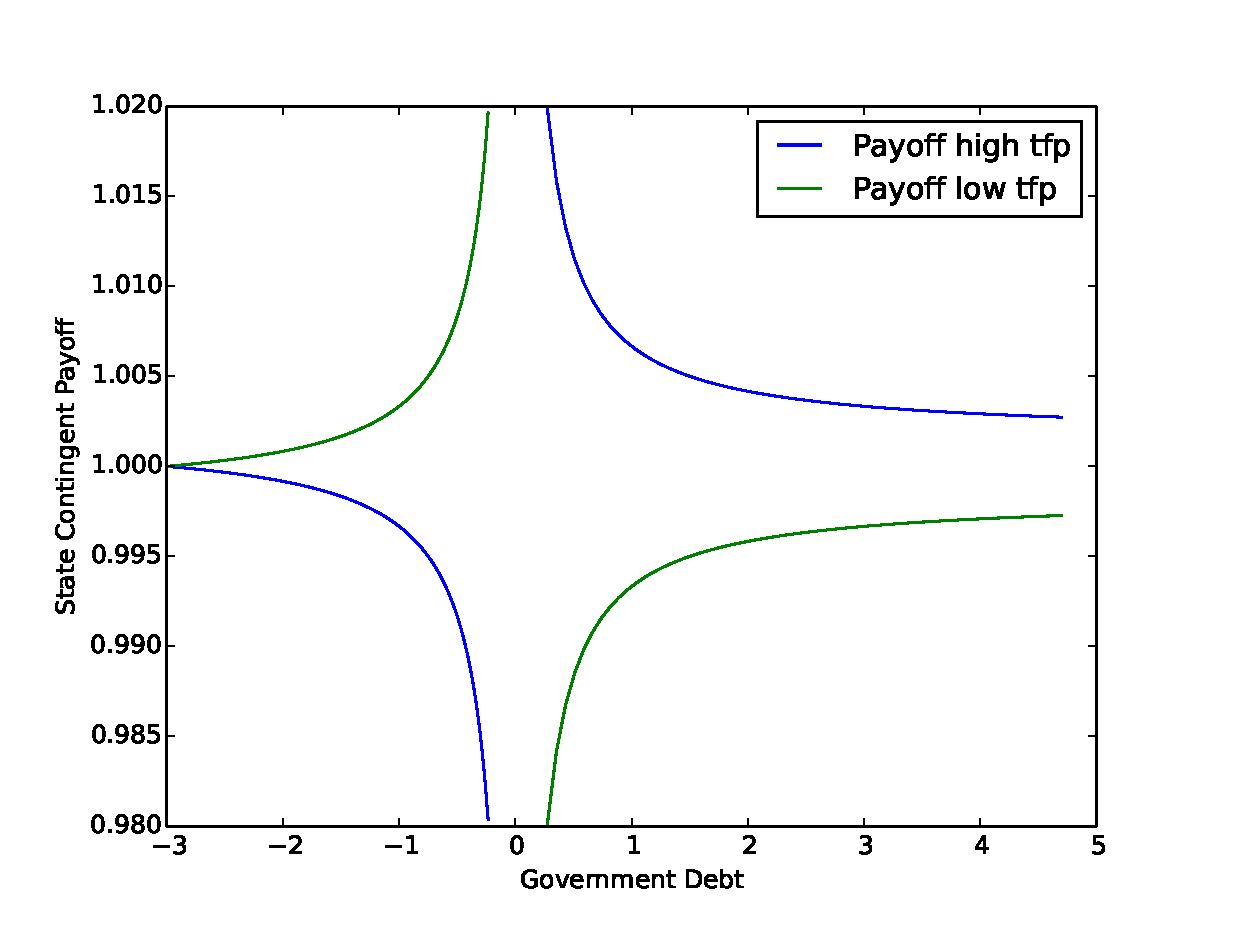
\includegraphics[scale=.4]{Images/p_graph_tfp.eps}
		\caption{Optimal asset payoff structure as a function of initial government debt when TFP follows a 2 shock i.i.d process}
	\end{center}	
	\end{figure}

  \end{frame}

%
  \begin{frame}
   \frametitle{Optimal Payoff Structure: Expenditure shocks}
	\begin{figure}
		\begin{center}
		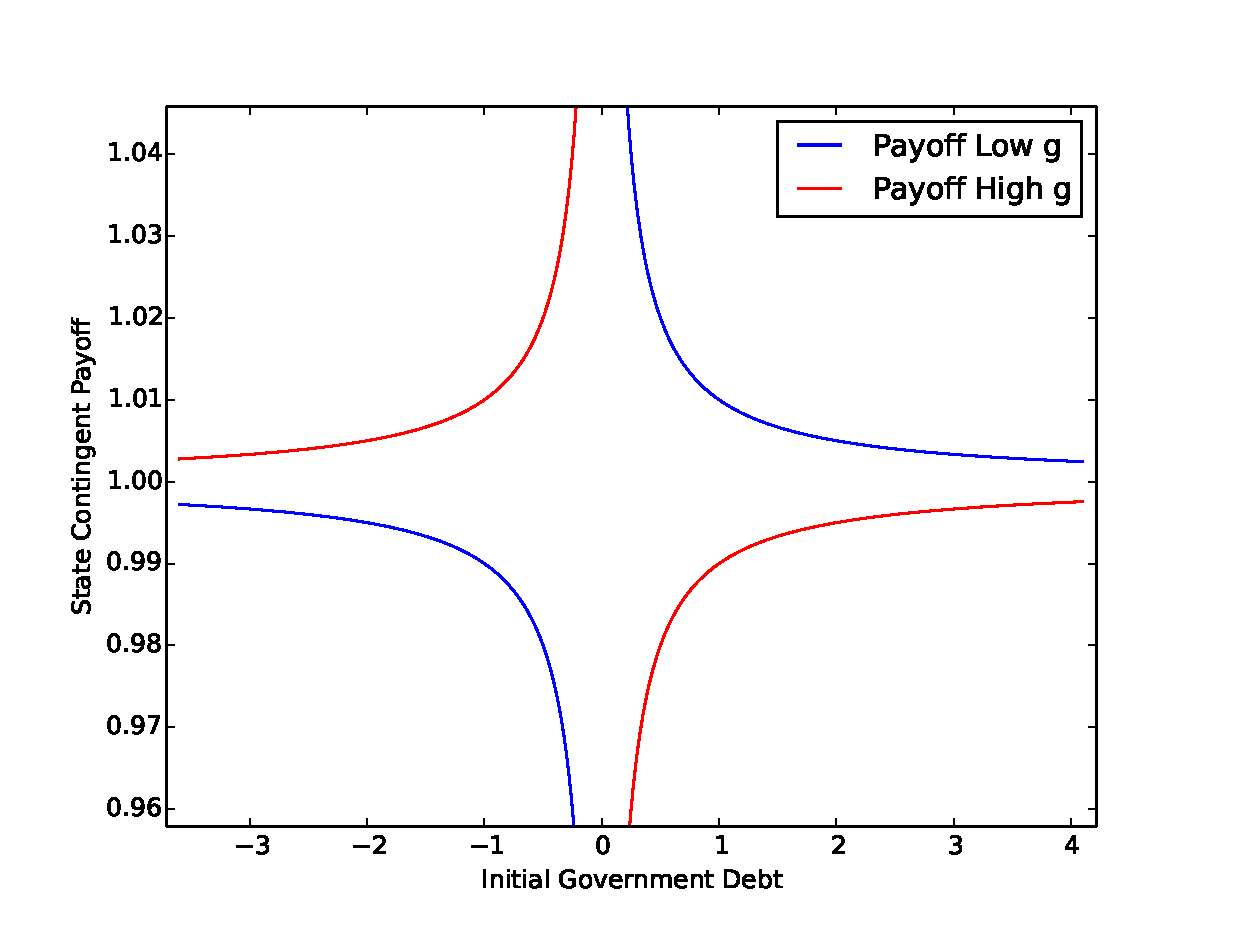
\includegraphics[scale=.4]{Images/p_graph.eps}
		\caption{Optimal asset payoff structure as a function of initial government debt when government expenditures follow 2 shock i.i.d process}
	\end{center}	
	\end{figure}

  \end{frame}
%
%


%
\begin{frame}
	\frametitle{Inverting the $\mathbb{P}^*$ mapping}
	\begin{enumerate}
		\item  \textbf{Exogenous payoff structure:} Suppose $\mathbb{P}\neq \mathbb{P}^*(b_{-1})$
		
		\item \textbf{Steady States: } A steady state is a government debt level  $b^*$ such that
		\[b_{t}=b^* \text{ implies } b_{t+\tau}=b^*\quad \forall \tau >0\]
	
			
		\item \textbf{Characterization: } Given an asset payoff structure $\mathbb{P}$
		\begin{itemize}
			\item Does a steady state exist? Is it unique?
			\item Value of $b^*$?
			\item For what levels of  \emph{initial government debt} $b_{-1}$ does  $b_t$ converge to $b^*$?
 			\end{itemize}
	\end{enumerate}
\end{frame}



 \begin{frame}
  \frametitle{Existence and $\mathbb{P}^{* -1}$}


 When shocks are i.i.d and take two values

  \begin{enumerate}

\item $\mathbb{P}(s|s\_)$ is independent of $s\_$ (so $\mathbb{P}$ can be a vector)
\item We can normalize $\mathbb{E}\mathbb{P}(s)=1$ and  then pin down payoffs with a scalar $\bm{p}$.
\begin{itemize}
 \item $\bm{p}$ is the payoff in the ``good'' state $s$
 \item A risk-free bond is a security for which $\bm{p}=1$
\end{itemize}

\item A steady state is obtained by inverting the optimal payoff mapping $p^*$
\begin{equation*}
\label{eq-ss}
b^* \ \textrm{satisfies} \  \bm{p}=\bm{p}^*(b^*) \ \textrm{or} \ p^{* -1}(p) = b^*
\end{equation*}

One equation in one unknown $b^*$
\end{enumerate}
\end{frame}



\begin{frame}
\frametitle{Existence regions in $\bm{p}$ space}

The payoff $\bm{p}$ in good state
$\in (0,\infty)$.

We can decompose a set of economies with different asset payoffs into 3 regions via thresholds $\alpha_2\geq\alpha_1\geq1$



  \begin{itemize}
   \item Low enough $\bm{p}(\leq \alpha_1$): government holds assets in steady state
   \item High enough $\bm{p} (\geq \alpha_2$): government  issues debt  in steady state
   \item Intermediate $\bm{p} (\alpha_1>\bm{p}>\alpha_2$): steady state does not exist
  \end{itemize}

 \end{frame}




\begin{frame}
 \frametitle{Thresholds: $\alpha_1 <\alpha_2$}
	%For either a pure TFP shock or a pure government expenditure shock,  we compute % $\alpha_1$ and $\alpha_2$ directly
	\begin{itemize}
		\item With only government expenditure shocks
		\[
			\alpha_1 = 1 \text{  and }  \alpha_2 = (1-\beta)\frac{\theta^\frac{\gamma}{1+\gamma}\left(\frac{1}{1+\gamma}\right)^\frac1\gamma\frac{\gamma}{1+\gamma}-g(s_1)}{\theta^\frac{\gamma}{1+\gamma}\left(\frac{1}{1+\gamma}\right)^\frac1\gamma\frac{\gamma}{1+\gamma}-\EE g} +\beta>1
		\]
		\item With only TFP shocks
		\[
			\alpha_1 = (1-\beta)\frac{\theta(s_1)^\frac{\gamma}{1+\gamma}}{\EE\theta^\frac{\gamma}{1+\gamma}}+\beta > 1
		\]and
		\[
		\alpha_2 = (1-\beta)\frac{\theta(s_1)^\frac{\gamma}{1+\gamma}\left(\frac{1}{1+\gamma}\right)^\frac1\gamma\frac{\gamma}{1+\gamma}-g}{\EE\theta^\frac{\gamma}{1+\gamma}\left(\frac{1}{1+\gamma}\right)^\frac1\gamma\frac{\gamma}{1+\gamma}-g}+\beta>\alpha_1
		\]
	\end{itemize}
 \end{frame}


\begin{frame}
   \frametitle{Existence regions in $\bm{p}$ space}
	\begin{figure}
		\begin{center}
		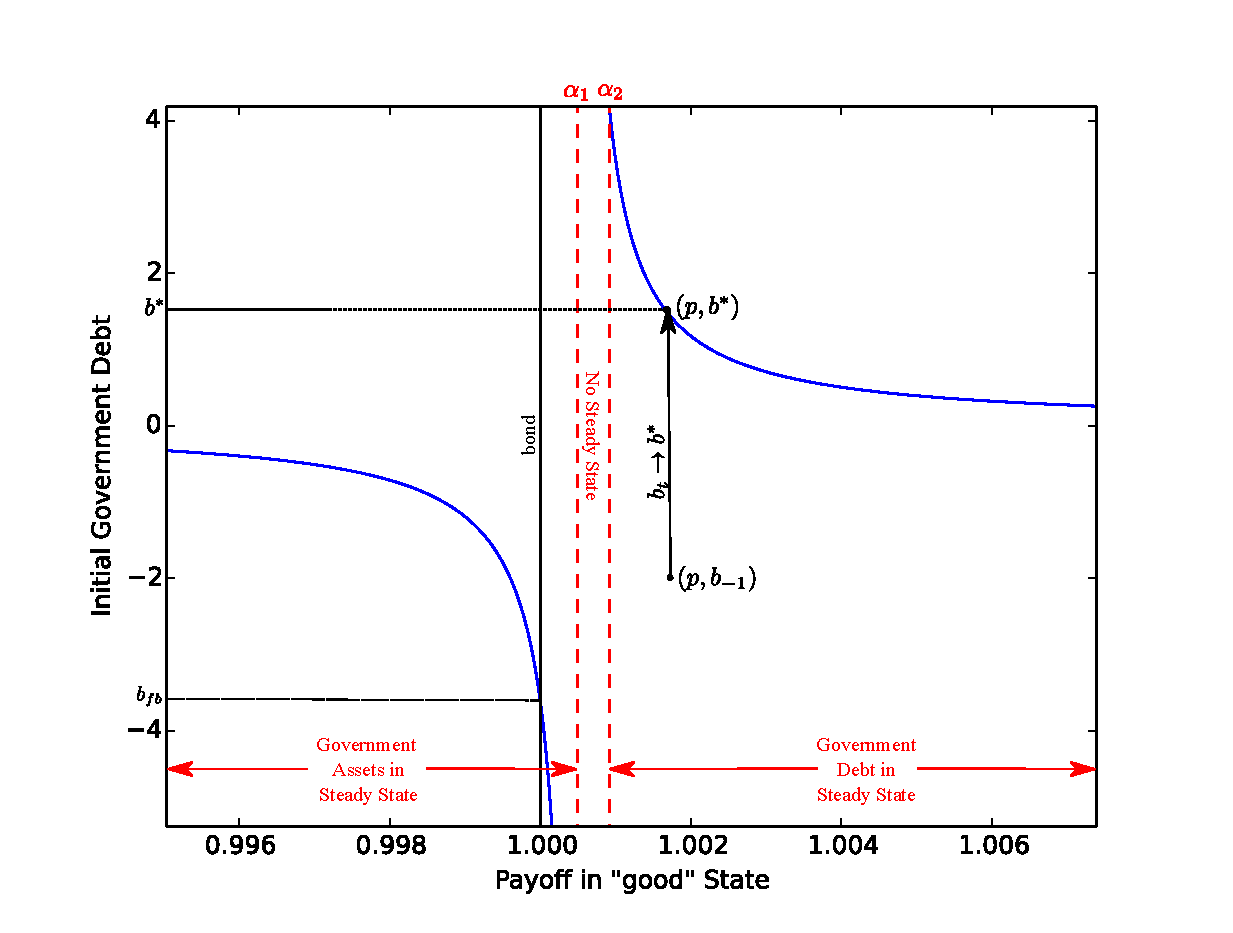
\includegraphics[scale=.5]{Images/graph_nostable.eps}
	\end{center}	
	\end{figure}

  \end{frame}


 \begin{frame}
  \frametitle{Convergence}
  \begin{itemize}
		\item Our analysis verifies existence of a steady state in a 2-state i.i.d. economy.
		\item To study long-run properties of a Ramsey allocation, we want to know whether steady state is stable
		\item \textbf{Risk-adjusted martingale:}
		
		The Lagrange multiplier $\mu_t$ on the implementability  constraint   satisfies
		\[
			\mu_t = \EE_t p_{t+1} \mu_{t+1}
		\] or
		\[
		\EE_t  \mu_{t+1}	= \mu_t -Cov_t (p_{t+1}, \mu_{t+1})
		\]
			%\emph{$\mu_t$ follows a risk adjusted martingale.}
	
		\item \textbf{Stability criterion: }   Away from a steady state, is the drift  of $\mu_t$ big enough?
		\end{itemize}
	

  \end{frame}

  \begin{frame}
  \frametitle{Characterizing convergence under quasi-linearity, iid, and $S=2$}

  \begin{itemize}
  \item Reminder:  $\bm{p}$ is the payoff in the ``good'' state.
   \item We partition  the ``$\bm{p}$ space'' into stable and unstable regions
     \end{itemize}

 	\begin{theorem}
Let $b^*$ denote the steady state level of govt.  debt and $b_{fb}$ be the level of debt that  supports the first-best allocation with complete markets.  Then % for  same $  \alpha_1 < \alpha_2$
		\begin{enumerate}
			\item  \textbf{Low $\bm{p}$}: If $\bm{p}\leq\min(\alpha_1,1)$ then  $b_{fb}<b^*<0$ and $b_t\rightarrow b^*$ with probability 1.
			\item \textbf{High  $\bm{p}$}:  If $\bm{p} \geq \alpha_2$ then   $0<b^*$ and $b_t \rightarrow b^*$ with probability 1.
			
			
			\end{enumerate}
			\end{theorem}
			
			For the intermediate region where  $b^*$ either does not exist or is unstable, there is a tendency to run up debt
		
		
	
 \end{frame}


\begin{frame}
   \frametitle{Stability regions}
	\begin{figure}
		\begin{center}
		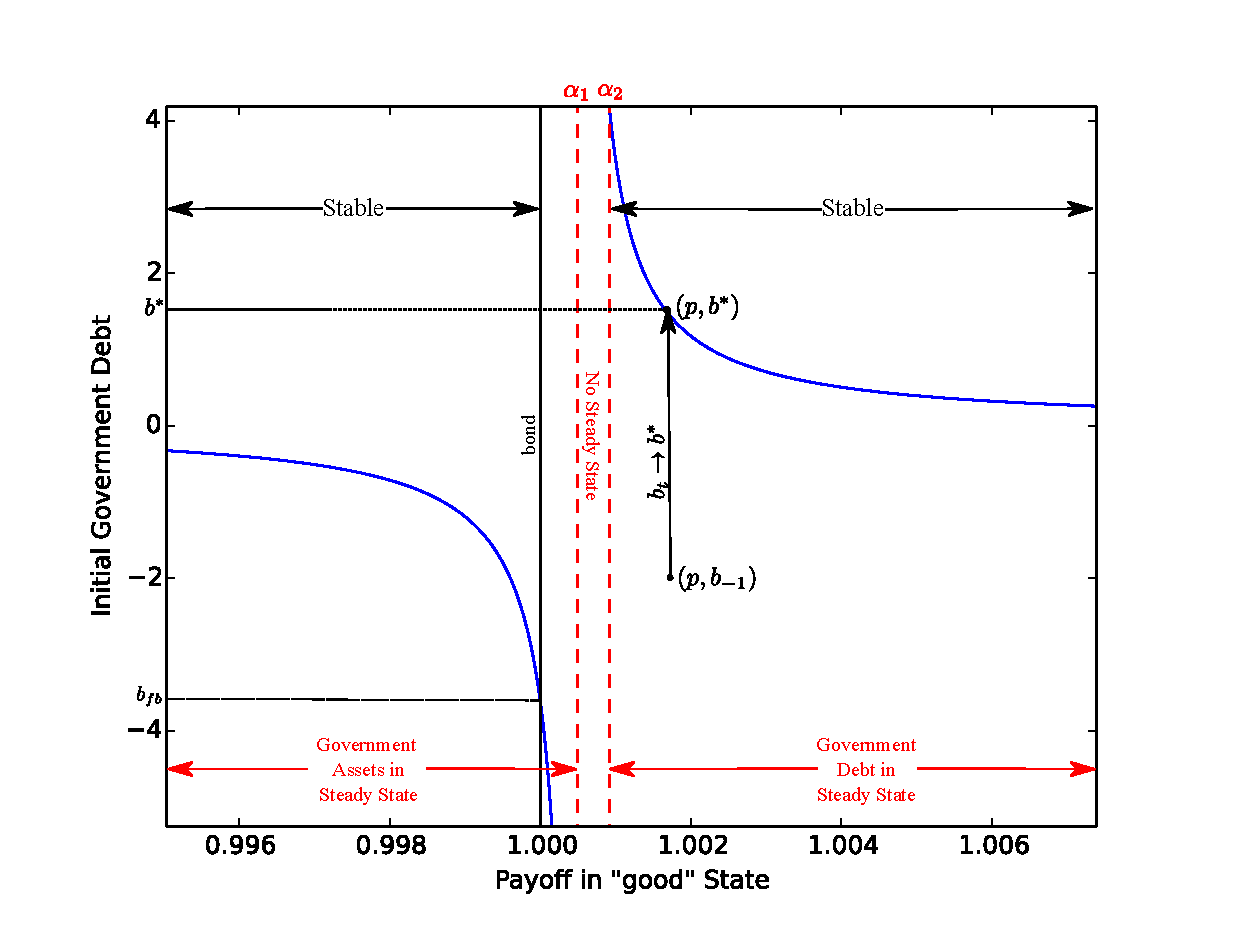
\includegraphics[scale=.5]{Images/graph_stable.eps}
	\end{center}	
	\end{figure}

  \end{frame}


 \begin{frame}

	\frametitle{A sample path with  $\bm{p} > 1$}
	\begin{center}
	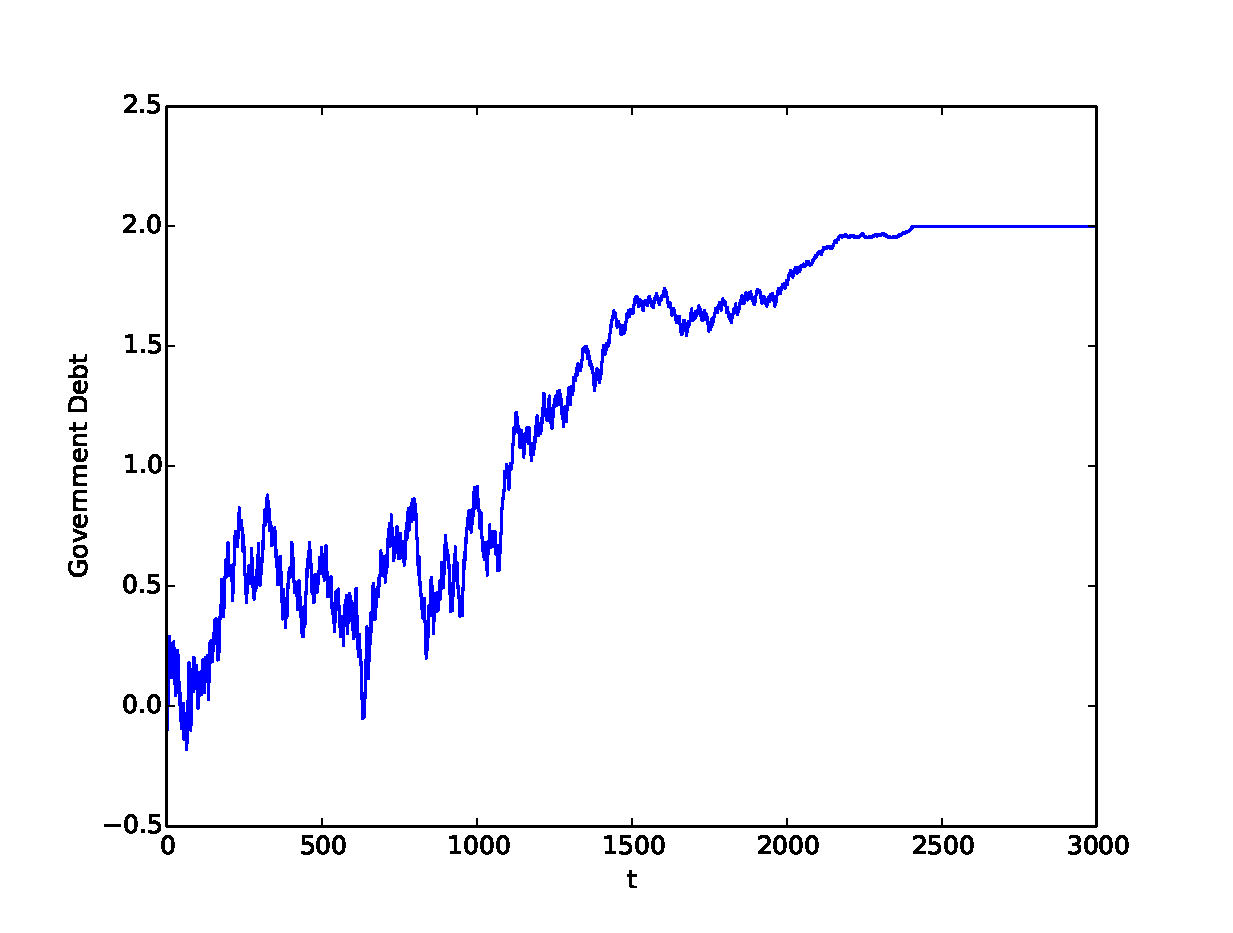
\includegraphics[width=4in]{Images/port1.eps}
	\end{center}
\end{frame}

\begin{frame}
	\frametitle{A sample path with   $\bm{p} <1$}
	\begin{center}
	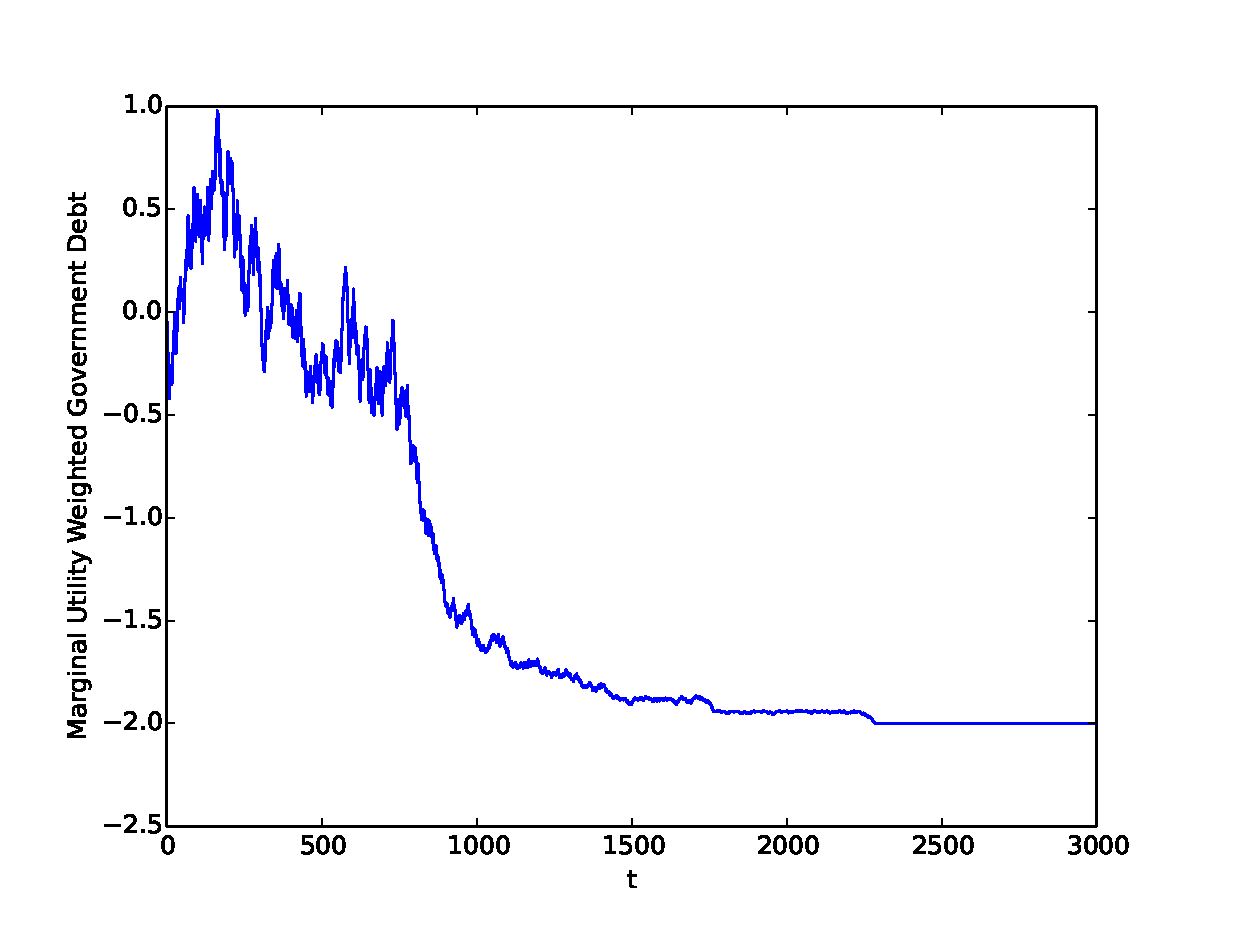
\includegraphics[width=4in]{Images/port2.eps}
	\end{center}
\end{frame}
%
% \begin{frame}
% 	\frametitle{Intuition and Generalizations}
% 	\begin{enumerate}
% 		\item The intuition we gain from our 2-state example is that, given exogenous payoff restrictions on government debt, there exist debt positions that allow the government to better smooth tax distortions across states.
% 		\item  Over time, the government adjusts it's debt position in order to best reallocate resources across states.
% 		\item  \textbf{Extensions: } more general preferences and more general aggregate state processes.
% 		\begin{itemize}
%
% 		\item  With risk aversion we are able to obtain similar results under the 2 state i.i.d assumption.
% 		\item More general processes require us to develop computational tools to analyze the long run dynamics
% 		\end{itemize}
%
% 		%\item  For more general aggregate state processes there no longer exists a complete markets %steady state.
% 		%\item  This requires us to develop computational tools to analyze the long-run dynamics.
% 		%\item  We find that with more general processes there exist regions with low volatility, because the government's debt position is reallocating resources across states and in the long run the government debt converges to these regions.
% 	\end{enumerate}
% \end{frame}
% %
\begin{frame}
 \frametitle{Outcomes with quasi-linear preferences}
 \textbf{Outcomes:}
 \begin{enumerate}
  \item  Often $b_t\to b^*$ when the aggregate state follows a 2-state i.i.d. process
  \item The level  and sign of $b^*$ depend on the \textbf{exogenous payoff structure} $\mathbb{P}$
  \item The limiting allocation corresponds to a complete market Ramsey allocation for initial govt. debt $b^*$
 \end{enumerate}

 \end{frame}



 \begin{frame}{Turning on risk-aversion}
  \textbf{Modifications:}
  \begin{itemize}
  \item Another source of return fluctuations -- the risk-free interest rate
   \item Marginal utility adjusted debt  encodes history dependence
   \item  With binary i.i.d shock shock process,  $x_t=u_{c,t}b_{t}$  converges

   \item Long-run properties of $x_t$ depend on equilibrium returns $R_{t,t+1}=\frac{\mathbb{P}(s_{t+1}|s_t)}{q_t(s^t)}$.
   Now $q_t$ varies in interesting ways


  \end{itemize}
  %\emph{To retain analytical tractability and clarify our analysis we will remove exogenous fluctuations in the payoff terms by restricting $p(s) =1$}
  \end{frame}
%


\begin{frame}
\frametitle{Roadmap, II}


 Two subproblems
\begin{enumerate}
 \item  $t=0$ Bellman equation in value function $W(b_{-1},s_0)$ %\textcolor{red}{Anmol and David XXXXXX: I altered the notation}
 \item  $t\geq 1$ Bellman equation in value function $V(x,s\_)$
\end{enumerate}

Seek steady states $x^*$ such that $x_t \to x^*$

\end{frame}




 \begin{frame}
	\frametitle{A Recursive Formulation}
	
	\begin{enumerate}
	 \item Commitment implies that government actions at $t \geq 1$ are constrained by the public's anticipations about them at $s < t$
	 \item This contributes additional state variables like marginal utility of consumption
	 \item Scaling the budget constraint by marginal utility makes Ramsey problem  recursive in  $x=U_c b$
	
	\[
		\frac{x_{t-1} p_t U_{c,t}}{\beta \EE_{t-1} p_t U_{c,t}}  = U_{c,t}c_t+U_{l,t} l_t + x_t
	\]
	
	%\item The planner's problem recursively with a single state variable.
	\end{enumerate}
	
	
	\end{frame}
	\begin{frame}
	\frametitle{Bellman equation for $t\geq1$ (\textit{ex ante})}
	\[
		V(x,s\_) = \max_{c(s),l(s),x'(s)} \sum_s \Pi(s,s\_)\Bigl(U(c(s),l(s)) + \beta V(x'(s),s)\Bigr)
	\]subject to $x'(s)\in [\underline x,\overline x]$
	\begin{align*}
		\frac{x \mathbb{P}(s) U_c(s)}{\beta\EE \mathbb{P}Uc} =U_c(s)c(s)+U_l(s)l(s) + x'(s)\\
		c(s) + g(s) = \theta(s)l(s)
	\end{align*}
	
 \end{frame}
\begin{frame}
	\frametitle{Time $0$ Bellman equation (\textit{ex post})}
	Given an initial  debt $b_{-1}$, state $s_0$,  and continuation value function $V(x,s\_)$
%\textcolor{red}{Anmol and David XXXXX: I altered the below by adding the $W$ function; but there is a problem with the timing of
%the $b$ argument.  See earlier slide where $W$ is defined.}
	\[
		W(b_{-1},s_0) = \max_{c_{0},l_0,x_{0}} U(c,l) +\beta V(x_0,s0)
	\]subject to  time zero implementability constraint
	\[
		U_{c}(c_0,l_0)c + U_l(c_0,l_0) l_0 + x_0 = U_c(c_0,l_0) b_{-1}
	\]and  resource constraint
	\[
		c_0+ g(s_0) = \theta(s_0) l_0
	\]and
	\[
		x_0 \in [\underline x,\overline x]
	\]
\end{frame}



\begin{frame}{Progress report}

\begin{enumerate}
 \item  Existence proved only under a special case of a risk-free bond  $\mathbb{P}(s|s\_)=1 \ \forall \ (s,s\_)$

 This focuses attention  on \textit{endogenous} component of returns coming from $q_t(s^t)$

 \item   $x^*$  is an initial condition for which the optimal asset payoff  in a LS economy is a risk-free bond

\end{enumerate}

\end{frame}

\begin{frame}
 \frametitle{Revisiting steady states with risk aversion}
Let $x'\left( s;{x},s\_\right) $ be an optimal  law of motion for the state variable
for the $t\geq1$ recursive problem.

\begin{definition}
 A steady state  ${x}^{*} $  satisfies ${ x}^{*}  =x' \left( s;{x}^{*},s_{-}\right) $ for all $%
\,s,s\_$
\end{definition}


\vspace{3mm}
\emph{Thus, a steady state is a node at which  continuation allocation and tax rate have no further history dependence. }

 \end{frame}




 \begin{frame}
	\frametitle{Existence}
	
	\begin{enumerate}
	 \item For a class of economies with separable iso-elastic preferences
	 $U(c,l) = \frac{c^{1-\sigma}}{1-\sigma} -\frac{ l^{1+\gamma}}{1+\gamma}$
	 \item Shocks that take two values and are i.i.d with $s_b$  being the ``adverse'' state (either low TFP or high expenditure)
	\end{enumerate}

	
	Let $x_{fb}$ be a value of the state $x$ from which a government can implement first=best with complete markets
	
	
	
	
	\begin{proposition}  Let $q_{fb}(s)$ be the shadow price of government debt in state $s$ using the first best allocation.
	If
	\[
		\frac{1-q_{fb}(s_b)}{1-q_{fb}(s_g)} > \frac{g(s_b)}{g(s_g)}>1
	\]
	
	Then there exists a steady state with $x_{fb}>x^*>0$
		\end{proposition}
\end{frame}


%



%
%
%
% \begin{frame}
% 	\frametitle{A Recursive Approach: Time 0}
% 	Given the initial debt level $b_0$, state $s_0$,  and the continuation value function $V(x,s\_)$ the planner's problem is then to solve the following
% 	\[
% 		\max_{c,l,x'} U(c,l) +\beta V(x',s0)
% 	\]subject to the time zero implementability constraint
% 	\[
% 		U_{c}(c,l)c + U_l(c,l) l + x' \geq U_c(c,l) b_0
% 	\]and the resource constraint
% 	\[
% 		c+ g(s_0) = \theta l
% 	\]and
% 	\[
% 		x' \in [\underline x,\overline x]
% 	\]
% \end{frame}
%
%
% %
% %   \item With risk aversion
% %   \item  To clarify our analysis we will remove exogenous fluctuations in the payoff terms $p_t U_{c,t}$ by restricting $p_t =1$.
% %  \end{enumerate}
% %
% % 	      \item quasilinear analysis found that there existed steady states when the aggregate state followed a 2 -state i.i.d. process.
% % 		\item Marginal utility weighted debt $x_t b_t U_{c,t}$ indexes the the space of optimal allocations with state contingent debt
% % 		\item  We would therefore expect a steady states to exist for the variable $x$
% % 		\item  To clarify our analysis we will remove exogenous fluctuations in the payoff terms $p_t U_{c,t}$ by restricting $p_t =1$.
% % 		\begin{itemize}
% % 			\item  Note under this restriction the endogenous payoff terms will be larger in bad states of the world, and thus, the government will hold assets in the steady state
% % 		\end{itemize}
% % 	\end{itemize}
% %\end{frame}
%
%
% \begin{frame}
% 	\frametitle{Incomplete Market's with Risk Aversion}
% 	\begin{itemize}
% 	\item By choosing a new variable $x_{t-1} = b_{t-1} U_{c,t-1}$ the measurability constraints can be written as a period by period constraint
% 	\[
% 		\frac{x_{t-1} p_t U_{c,t}}{\beta \EE_{t-1} p_t U_{c,t}}  = U_{c,t}c_t+U_{l,t} l_t + x_t
% 	\]
% 	\item  This bares a striking resemblance to the period by period constraint for quasi-linear preferences
% 	\[
% 		\frac{b_{t-1} p_t}{\beta \EE_{t-1} p_t} = c_t + U_{l,t} l_t + b_t
% 	\]
% 	\item  The $p_tU_{c,t}$ terms in the risk averse budget constraint act as endogenous payoffs.
% 	\end{itemize}
% \end{frame}
%
%  \begin{frame}
% 	\frametitle{Existence}
% 	Let $x_{fb}$ be the $x$ with which the government can institute first best from that period onwards.  Assume a CRRA utility specification $U(c,l) = \frac{c^{1-\sigma}}{1-\sigma} -\frac{ l^{1+\gamma}}{1+\gamma}$.  Finally, let  $c_{fb}$ and $l_{fb}$ be consumption and leisure under first best.  We have the following proposition
% 	\begin{proposition}  For a 2 state i.i.d. process let  $s_g$ and $s_b$ denoting the states with high and low consumption at first best.  If
% 	\[
% 		\frac{g(s_g)}{1-\frac{\beta\EE[(c_{fb})^{-\sigma}]}{c_{fb}(s_g)}} > \frac{g(s_b)}{1-\frac{\beta\EE[(c_{fb})^{-\sigma}]}{c_{fb}(s_b)}}
% 	\]  Then there exists a multiplier $\mu$ and complete markets solutions $c^\mu,l^\mu$ such that
% 	\[
% 	\underline x<\frac{U_{c_\mu}(s)c_\mu(s) + U_{l_\mu}(s) l_\mu(s)}{\frac{U_{c_\mu}(s)}{\beta\EE[U_{c_\mu}]}-1} = x^* <0
% 	\]
% 	\end{proposition}
% \end{frame}
%
%
\begin{frame}
	\frametitle{Stability}
	\begin{enumerate}
	 \item Here interest rates are aligned with marginal utility of consumption;  they are low  in ``good'' states (high TFP or low expenditure)
	 \item The government holds claims against the private sector in the steady state. Similar to the quasilinear case with  low  $\bm{p}$	
	 \item The incomplete markets Ramsey allocation converges to a Lucas-Stokey  Ramsey allocation for all initial conditions	 	
	\end{enumerate}


	\begin{proposition}  Let $\{c_t(s^t), l_t(s^t), x_t(s^{t-1})\}$ solve the incomplete markets Ramsey problem with $x_0 > x^*$.  Then  $x_t(s^{t-1})\rightarrow x^*$ as $t\rightarrow \infty$ with probability 1 for all initial conditions
	
	\end{proposition}
	\end{frame}
	
%
% \begin{frame}
% 	\frametitle{Quasilinear vs. risk aversion}
% 	{\color{red} Redo this slide}
% 	\begin{itemize}
% 				\item  With  quasilinear preferences and a risk-free bond, the interest rate is always $1/\beta$.
%    \item With risk averse preferences, interest rate is higher in periods of high government expenditure.
% 		\item  Thus, while the government has greater expenses in high government expenditure states, the higher interest rate means that the government can  accumulate less and still  cover future government expenditures.
% 		\item  After the government has accumulated enough assets, it is actually better off in periods of high government expenditure than in periods with low government expenditures (since its claims to consumption are worth more).
% 		\item  By holding assets, the government is able to reallocate resources across states, something it is not able to do in the quasilinear case.
% 	\end{itemize}
% \end{frame}
%
\begin{frame}
	\frametitle{A sample path for 2 state i.i.d. process with risk aversion}
	\begin{center}
	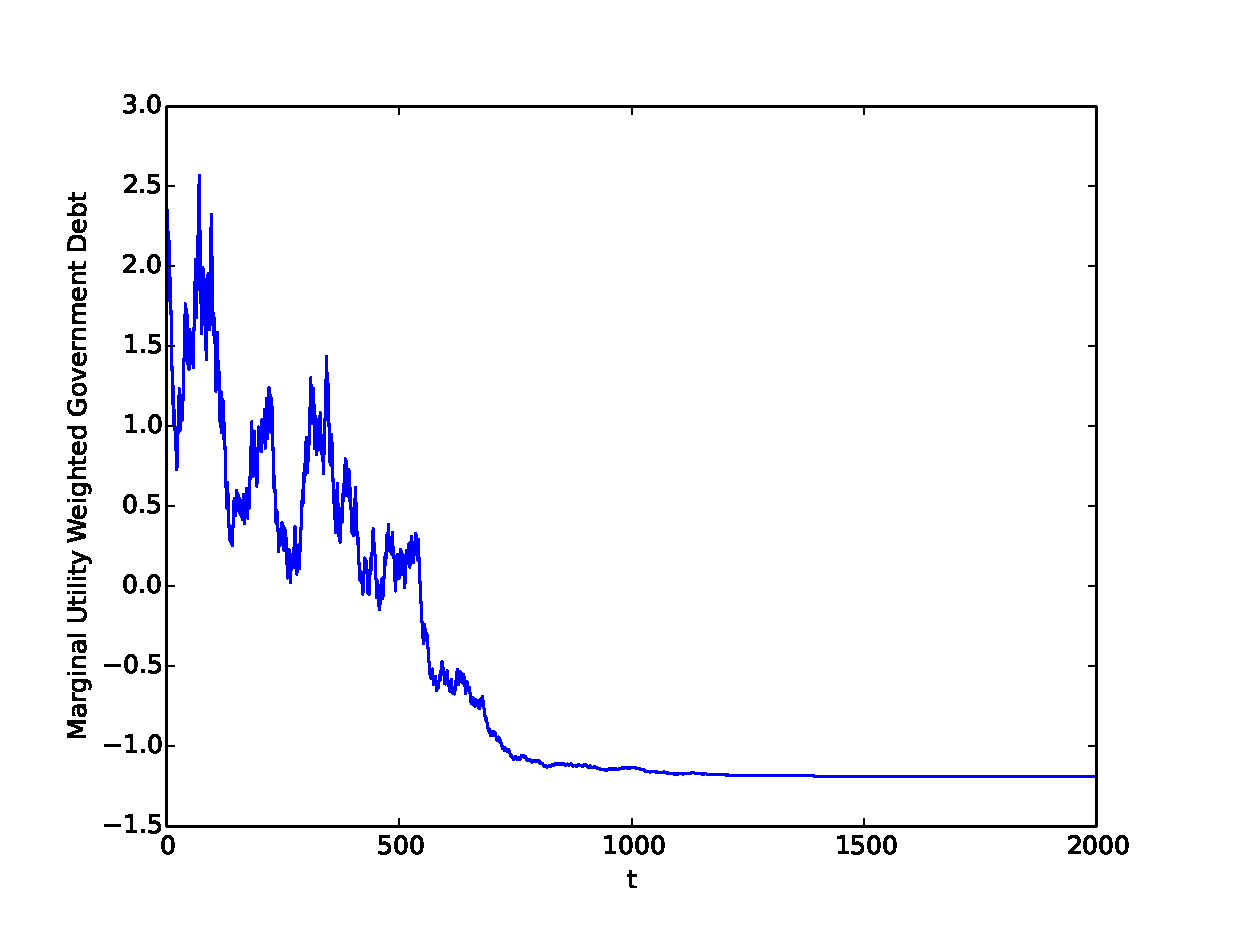
\includegraphics[width=4in]{Images/2stateiid.eps}
	\end{center}
\end{frame}

\section{Numerical Results}
\subsection{}

\begin{frame}
	\frametitle{A sample path  for economy with $S>2$ states}
	\begin{center}
	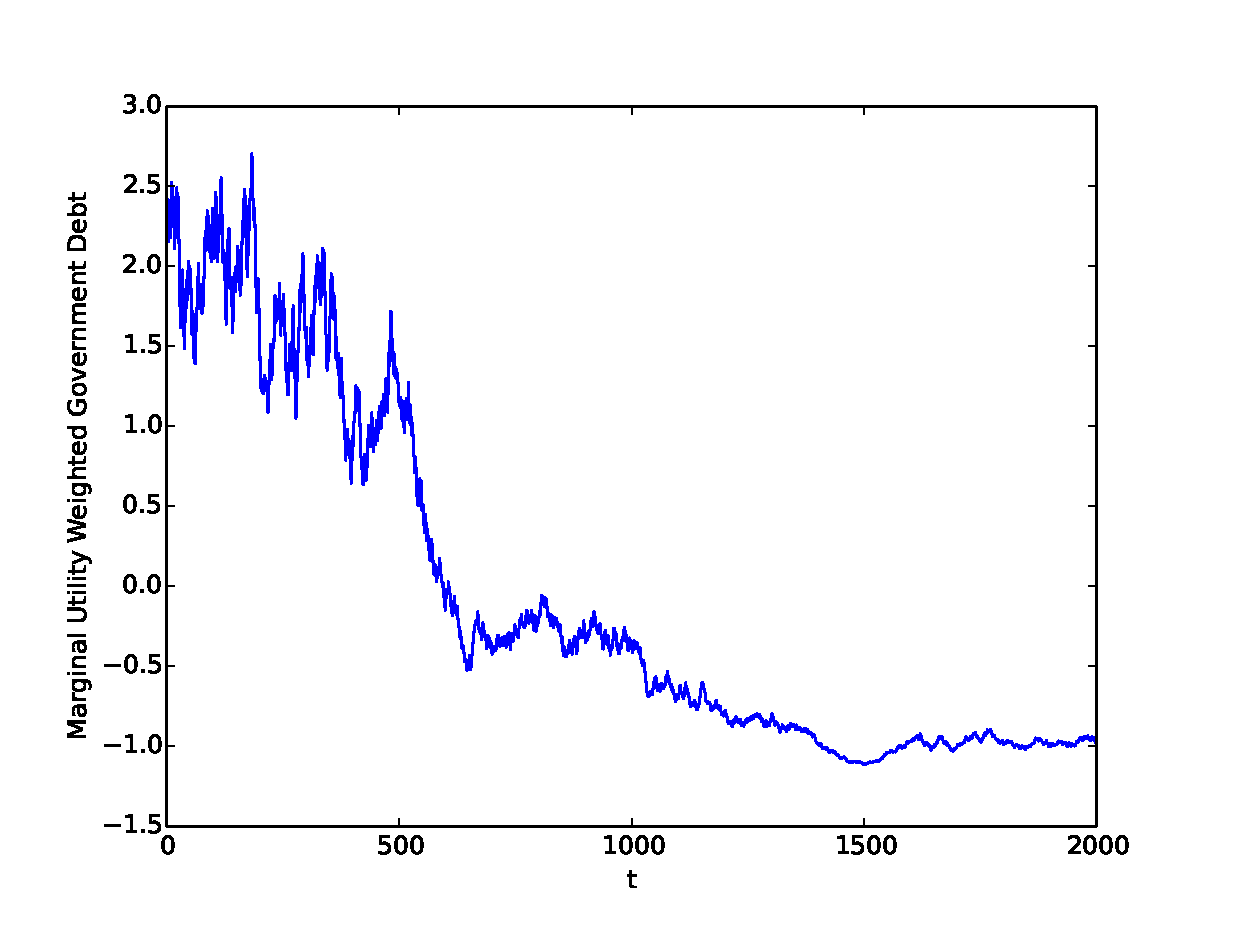
\includegraphics[width=4in]{Images/5stateiid.eps}
	\end{center}
\end{frame}



 \begin{frame}
  \frametitle{Transfers}
	\begin{itemize}	
	\item Access to nonnegative transfers makes first-best level of assets trivially a ``steady state''  	
\item  All results hold \textit{on one side} of steady state
\begin{theorem}

With nonnegative lump sum transfers,  in cases where a steady state exists and is stable,  if the initial debt of the government exceeds its steady state level,  the economy  converges with probability 1 to the steady state.

\end{theorem}
		
	\end{itemize}
 \end{frame}

 \begin{frame}
	\frametitle{Quasilinear preferences and risk-free bond  with and without nonnegative transfers}
	\begin{center}
	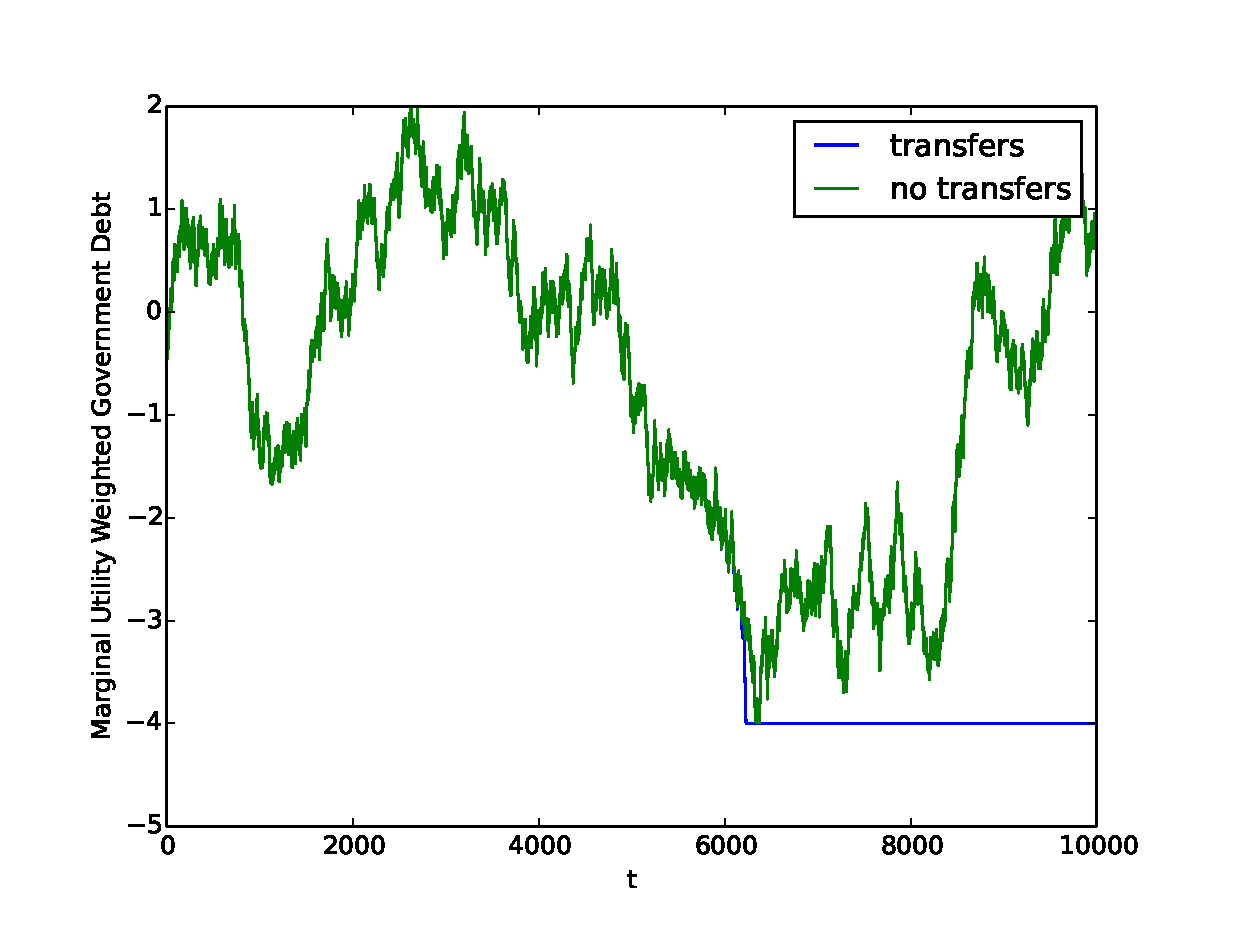
\includegraphics[width=4in]{Images/transfer_example2.eps}
	\end{center}
\end{frame}


%\begin{frame}{Battle field}
%\small
%\textit{What are the long run levels of government holdings ?}
%
%\vspace{3mm}
%
%With shocks that are IID and take two values,
%
%\begin{tabular}[h]{| l | p{1.25in} | p{1.25in} |}
%	\hline
%	&$p = 1$& $p\neq 1$\\
%	\hline
%	Quasi-Linear& (AMSS)
%	
%	With $T_t\geq 0$, hold assets at first best .&Partition the payoff space such that either
%	
%	a) issue or
%	b) run up debt eventually\\
%	\hline
%	Risk Aversion& Conditions under which
%	
%	assets $<$ first best& \emph{Conjecture:} Similar results  as in quasi-linear case\\
%	\hline
%\end{tabular}
%
%
%\vspace{4mm}
%
%In future work we plan to study more general shocks processes
%
%\end{frame}
\begin{frame}{Battle field}
\small
\textit{What is government debt in long-run?}


\vspace{3mm}

With shocks that are IID and take two values

\medskip


\begin{tabular}[h]{| l | p{1.25in} | p{1.25in} |}
	\hline
	&risk-free bond & risky bond \\
	\hline
	Quasi-Linear& (AMSS)
	
	With $T_t\geq 0$, govt. accumulates enough assets for first best.&Partition  payoff space so that govt. either
	
	a) issues or
	b) runs up debt eventually\\
	\hline
	Risk Aversion& Conditions under which limiting govt.	
	assets $<$ first best& \emph{Conjecture:} Similar to quasi-linear outcomes\\
	\hline
\end{tabular}


\vspace{4mm}

In future work we plan to study more general shocks processes

\end{frame}



\begin{frame}
 \frametitle{Comparison to literature}
 \begin{enumerate}
  \item Angelotos (2002), Buera and Nicolini (2004)

\begin{itemize}
 \item Begin with a complete market  Ramsey allocation
 \item Ask if this can be spanned by \emph{some} collection of non-contingents debt of different maturities?
\end{itemize}
\item This paper
\begin{itemize}
 \item Begin with an incomplete markets Ramsey allocation
 \item Ask whether the long-run allocation coincides with \emph{some} complete market allocation?
\end{itemize}

\item In BEGS1, we study a related problem with heterogeneous agents
\begin{itemize}
 \item We find ``steady states'' with constant labor taxes and ratios of consumptions
 \item But generically there do not exist initial assets and Pareto weights that  yield  stationary allocation
\end{itemize}



 \end{enumerate}


\end{frame}

 \begin{frame}
  \frametitle{Concluding remarks }
\begin{itemize}
	\item With market incompleteness, the asset payoff structure  has big implications a Ramsey government's  long run debt
	\item If the asset offers lower returns in adverse states of the world, the Ramsey government  asymptotically runs up a  debt to the private sector.
\item With risk aversion, cyclical properties of interest rate affects government debt asymptotically
	\item  Access to nonnegative transfers play little role in shaping outcomes.  Rather, the key  force is the government's ability to use its debt position to reallocate resources across states
	\item  \textbf{Future Research}:   With heterogeneous agents and unrestricted transfers, how does the type of market incompleteness affect long run wealth distributions and other outcomes?
\end{itemize}
 \end{frame}

  \end{document}
>>>>>>> a01df2b8b363f6c2690db010092b82416f93d208
%  